\section{Реализация}

Этапы реализации представлены в виде схемы (рис.~\ref{fig:fig1}). 
На первом этапе подключаются необходимые зависимости. 
На втором этапе проектируется и реализуется архитектура приложения (чистая архитектура + MVVM). 
На третьем этапе проектируется и разрабатывается пользовательский интерфейс. 
На четвертом этапе создается навигация между экранами в приложении. 
На пятом этапе добавляются сущности будущей базы данных.
Шестой этап включает в себя реализацию минимального серверного приложения.
Седьмой этап — проверка HTTP-запросов к серверному приложению. 
Восьмой этап — получение OpenSSL-сертификата для создания защищённого соединения.
Девятый этап — реализация логики синхронизации данных с серверным приложением.
Десятый этап — проектирование и реализация базы данных. 
Одиннадцатый этап — проектирование и реализация логики отображения тренировок, прогресса, сна и советов.
Двенадцатый этап — реализация модуля анализа тренировок и сна для формирования советов. 

\begin{figure}[htbp]
	\centering
	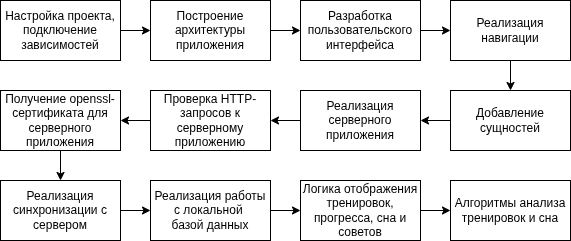
\includegraphics[width=1.0\textwidth]{images/diagrams/Этапы реализации.png}
	\caption{Схема этапов реализации приложения}
	\label{fig:fig1}
\end{figure}

\subsection{Подключение зависимостей}

Для написания приложения нужно добавить необходимые библиотеки в Gradle файле на уровне приложения: 
\begin{enumerate}
	\item Retrofit – библиотека для работы с HTTP-запросами. Используется для взаимодействия с собственным API, обеспечивая удобную отправку запросов и обработку ответов. Конвертер Gson автоматически преобразует JSON в объекты Kotlin.
	\item AndroidX Libraries – современные компоненты для Android-разработки.
	\item Jetpack Compose – декларативная верстка экранов.
	\item Jetpack Navigation – навигация между экранами.
	\item Koin – внедрение зависимостей, улучшает модульность и тестируемость.
	\item Room – работа с SQLite, хранение тренировок, упражнений, сна и истории.
\end{enumerate}

\subsection{Архитектура приложения}

Приложение разработано с соблюдением принципов чистой архитектуры, что обеспечивает высокую степень модульности, гибкости, тестируемости кода, а также упрощает поддержку и расширение функциональности \cite{refc}. Чистая архитектура разделяет систему на несколько слоёв, каждый из которых имеет чётко определённые задачи и зависимости (рис.~\ref{fig:clean_arch}):

\begin{figure}[H]
    \centering
    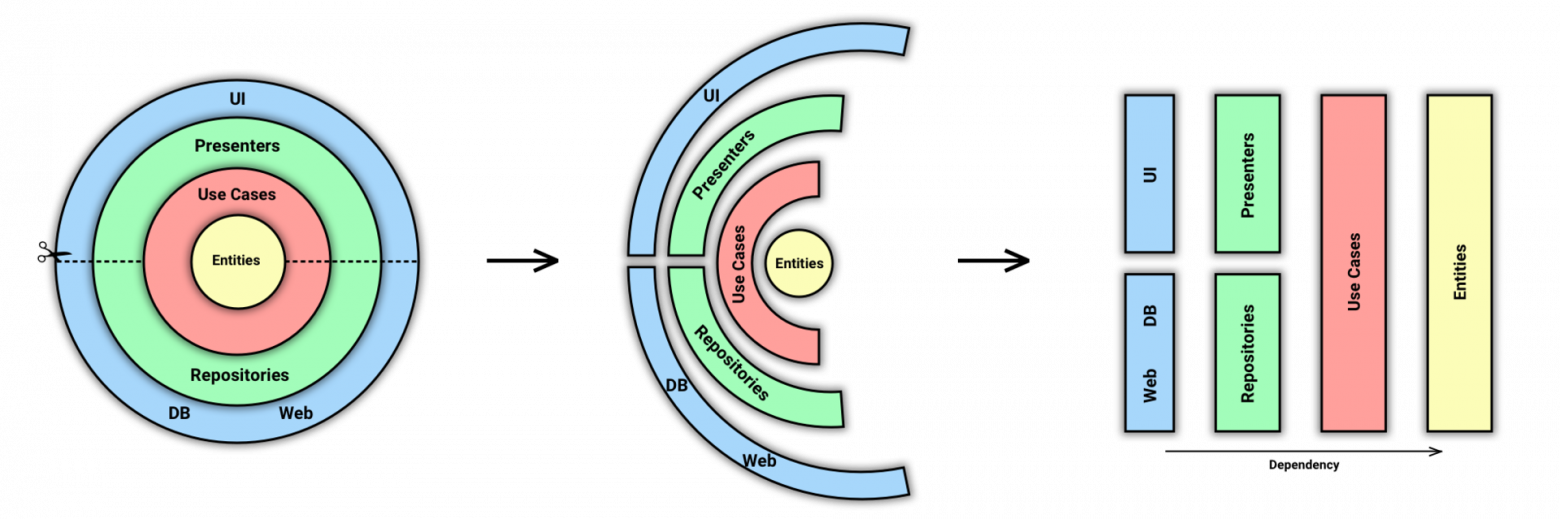
\includegraphics[width=1\textwidth]{images/diagrams/слои чистой архитектуры.png}
    \caption{Слои чистой архитектуры}
    \label{fig:clean_arch}
\end{figure}

\begin{enumerate}
    \item \textbf{Внешний слой (UI Layer)}: включает все компоненты, связанные с пользовательским интерфейсом, такие как фрагменты и активности. Основная задача UI Layer — отображение данных и взаимодействие с пользователем. Этот слой получает данные из ViewModel и обновляет интерфейс в соответствии с изменениями в данных \cite{refc}.
    \item \textbf{Слой данных (Data Layer)}: содержит компоненты, связанные с управлением данными, включая DAO-интерфейсы для работы с Room, реализации сетевых запросов с использованием Retrofit, а также клиентов базы данных и сетевых клиентов. Data Layer отвечает за получение и хранение данных, предоставляя их в Domain Layer через репозитории \cite{refc}.
    \item \textbf{Слой домена (Domain Layer)}: содержит бизнес-логику и бизнес-модели. Domain Layer не зависит от других слоев и содержит основные бизнес-правила и интерфейсы репозиториев \cite{refc}.
    \item \textbf{Слой приложений (Application Layer)}: содержит ViewModel, которые объединяют бизнес-логику с логикой представления и управления состоянием. ViewModel взаимодействуют с репозиториями для получения данных и обработки пользовательских действий.
\end{enumerate}

Для разделения представления и логики управления данными в приложении используется паттерн MVVM (Model-View-ViewModel). Этот паттерн (рис.~\ref{fig:mvvm}) обеспечивает чёткое разделение обязанностей между компонентами приложения:

\begin{figure}[H]
    \centering
    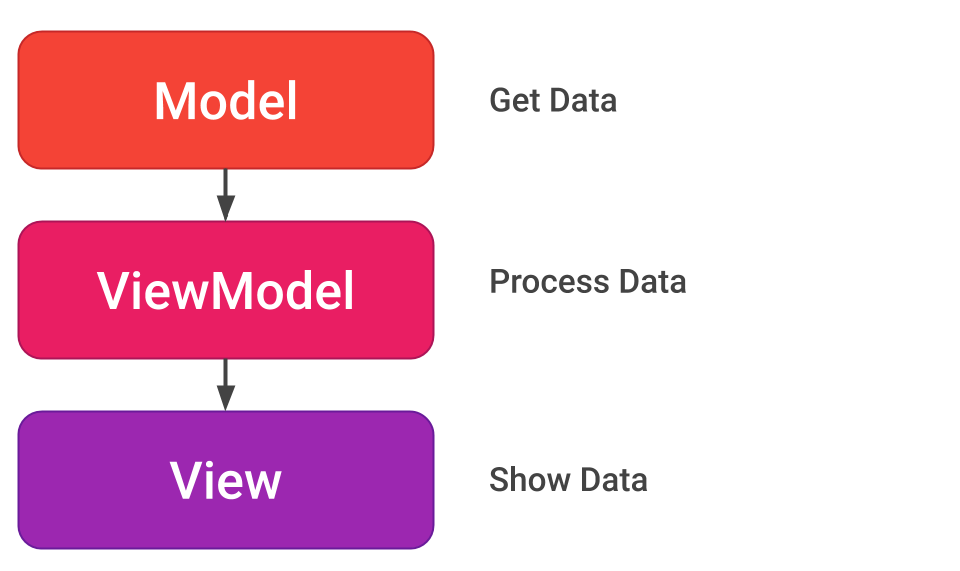
\includegraphics[width=1\textwidth]{images/diagrams/компоненты mvvm.png}
    \caption{Компоненты паттерна MVVM}
    \label{fig:mvvm}
\end{figure}

\begin{enumerate}
    \item \textbf{Model}: включает бизнес-логику и данные приложения. Модель получает данные из Data Layer и предоставляет их ViewModel.
    \item \textbf{View}: состоит из пользовательского интерфейса и отвечает за отображение данных. View наблюдает за изменениями в ViewModel и обновляет интерфейс в соответствии с этими изменениями.
    \item \textbf{ViewModel}: посредник между View и Model. ViewModel запрашивает данные у Model и предоставляет их View, а также обрабатывает пользовательские действия и обновляет Model.
\end{enumerate}

Для управления зависимостями и их внедрения в приложении используется библиотека Koin. В модулях Koin определяются зависимости и способы их создания. Например, можно определить зависимости для сетевого клиента, базы данных и ViewModel. Это позволяет централизованно управлять зависимостями и облегчает их модификацию. Koin автоматически предоставляет экземпляры классов, когда они требуются, что упрощает тестирование и модульность. Например, ViewModel могут получать необходимые репозитории через Koin, что устраняет жёсткие зависимости \cite{refj}.

\subsection{Структура проекта}

Проект организован в соответствии с принципами многомодульной архитектуры, что обеспечивает чёткое разделение ответственности, переиспользование кода и ускоряет сборку. Выделены следующие модули:

\begin{itemize}
    \item \texttt{app} — главный модуль приложения. Содержит точку входа (\texttt{Application} класс), основной манифест, ресурсы, а также конфигурацию сборки. В этом модуле происходит связывание остальных модулей и запуск приложения.
    
    \item \texttt{presentation} — модуль пользовательского интерфейса. Включает:
        \begin{itemize}
            \item экраны (\texttt{ui/screens/}) — каждый экран представлен отдельным пакетом;
            \item composable-функции, реализованные с помощью Jetpack Compose;
            \item ViewModel для каждого экрана, которые управляют состоянием UI и взаимодействуют с интеракторами (use cases) из доменного слоя;
            \item навигацию (Jetpack Navigation), объявленную в виде sealed-классов или навигационных графов.
        \end{itemize}
    
    \item \texttt{domain} — модуль доменного слоя (бизнес-логики). Не зависит от фреймворков Android и других модулей. Содержит:
        \begin{itemize}
            \item бизнес-модели (data-классы), например \texttt{Workout}, \texttt{Exercise}, \texttt{SleepRecord};
            \item интерфейсы локальных репозиториев: \texttt{LocalWorkoutRepository}, \texttt{LocalSleepRepository}, \texttt{LocalHistoryRepository}, \texttt{LocalUserRepository};
            \item интерфейсы удалённых репозиториев: \texttt{ExerciseRemoteRepository}, \texttt{HistoryRemoteRepository}, \texttt{WorkoutRemoteRepository}, \texttt{SleepRemoteRepository}, \texttt{UserRemoteRepository};
            \item use cases (интеракторы) — классы, реализующие отдельные сценарии: \texttt{GetWorkoutsUseCase}, \texttt{AddSleepRecordUseCase}, \texttt{GenerateRecommendationUseCase}.
        \end{itemize}
    
    \item \texttt{data} — модуль слоя данных. Реализует интерфейсы репозиториев, объявленные в \texttt{domain}, и управляет источниками данных (локальными и удалёнными). Структура модуля:
        \begin{itemize}
            \item \texttt{repository/} — реализации репозиториев: локальные реализации, включающие \texttt{LocalWorkoutRepositoryImpl}, \texttt{LocalSleepRepositoryImpl}, \texttt{LocalHistoryRepositoryImpl}, \texttt{LocalUserRepositoryImpl}; и удалённые реализации, включающие \texttt{ExerciseRemoteRepositoryImpl}, \texttt{HistoryRemoteRepositoryImpl},\texttt{WorkoutRemoteRepositoryImpl}, \texttt{SleepRemoteRepositoryImpl}, \text{UserRemoteRepositoryImpl}.
            \item \texttt{local/} — работа с локальной базой данных: Entity-классы, DAO, сама база данных (\texttt{AppDatabase});
            \item \texttt{remote/} — сетевые компоненты: DTO (Data Transfer Object), Retrofit-сервисы (\texttt{WorkoutApiService}, \texttt{SleepApiService}, \texttt{UserApiService} и др.);
            \item \texttt{mappers/} — функции преобразования между Entity, DTO и доменными моделями.
            \item \texttt{di} — пакет внедрения зависимостей, содержащий следующие модули:
            \texttt{networkModule} — предоставляет \texttt{OkHttpClient}, \texttt{Retrofit}, API-сервисы;
            \texttt{databaseModule} — предоставляет \texttt{AppDatabase} и DAO;
            \texttt{repositoryModule} — предоставляет реализации локальных и удалённых репозиториев;
        \end{itemize}
\end{itemize}

Такая организация соответствует рекомендациям Google по многомодульности и позволяет гибко масштабировать проект, изолированно тестировать каждый слой и переиспользовать доменную логику в других приложениях (например, в Wear OS или модульных тестах).

\subsection{Пользовательский интерфейс}

Все экраны приложения свёрстаны с помощью декларативного подхода Jetpack Compose. Для всех частей интерфейса используются стандартные UI-элементы Android SDK~\cite{refh}. Вынесены отдельно строковые и цветовые ресурсы, необходимые шрифты и векторные изображения для иконок. Добавлена поддержка светлой и тёмной темы.

Ниже представлены основные экраны приложения (рис.~\ref{fig:main}–\ref{fig:sleep}):

\begin{figure}[htbp]
    \centering
    \begin{minipage}{0.18\textwidth}
        \centering
        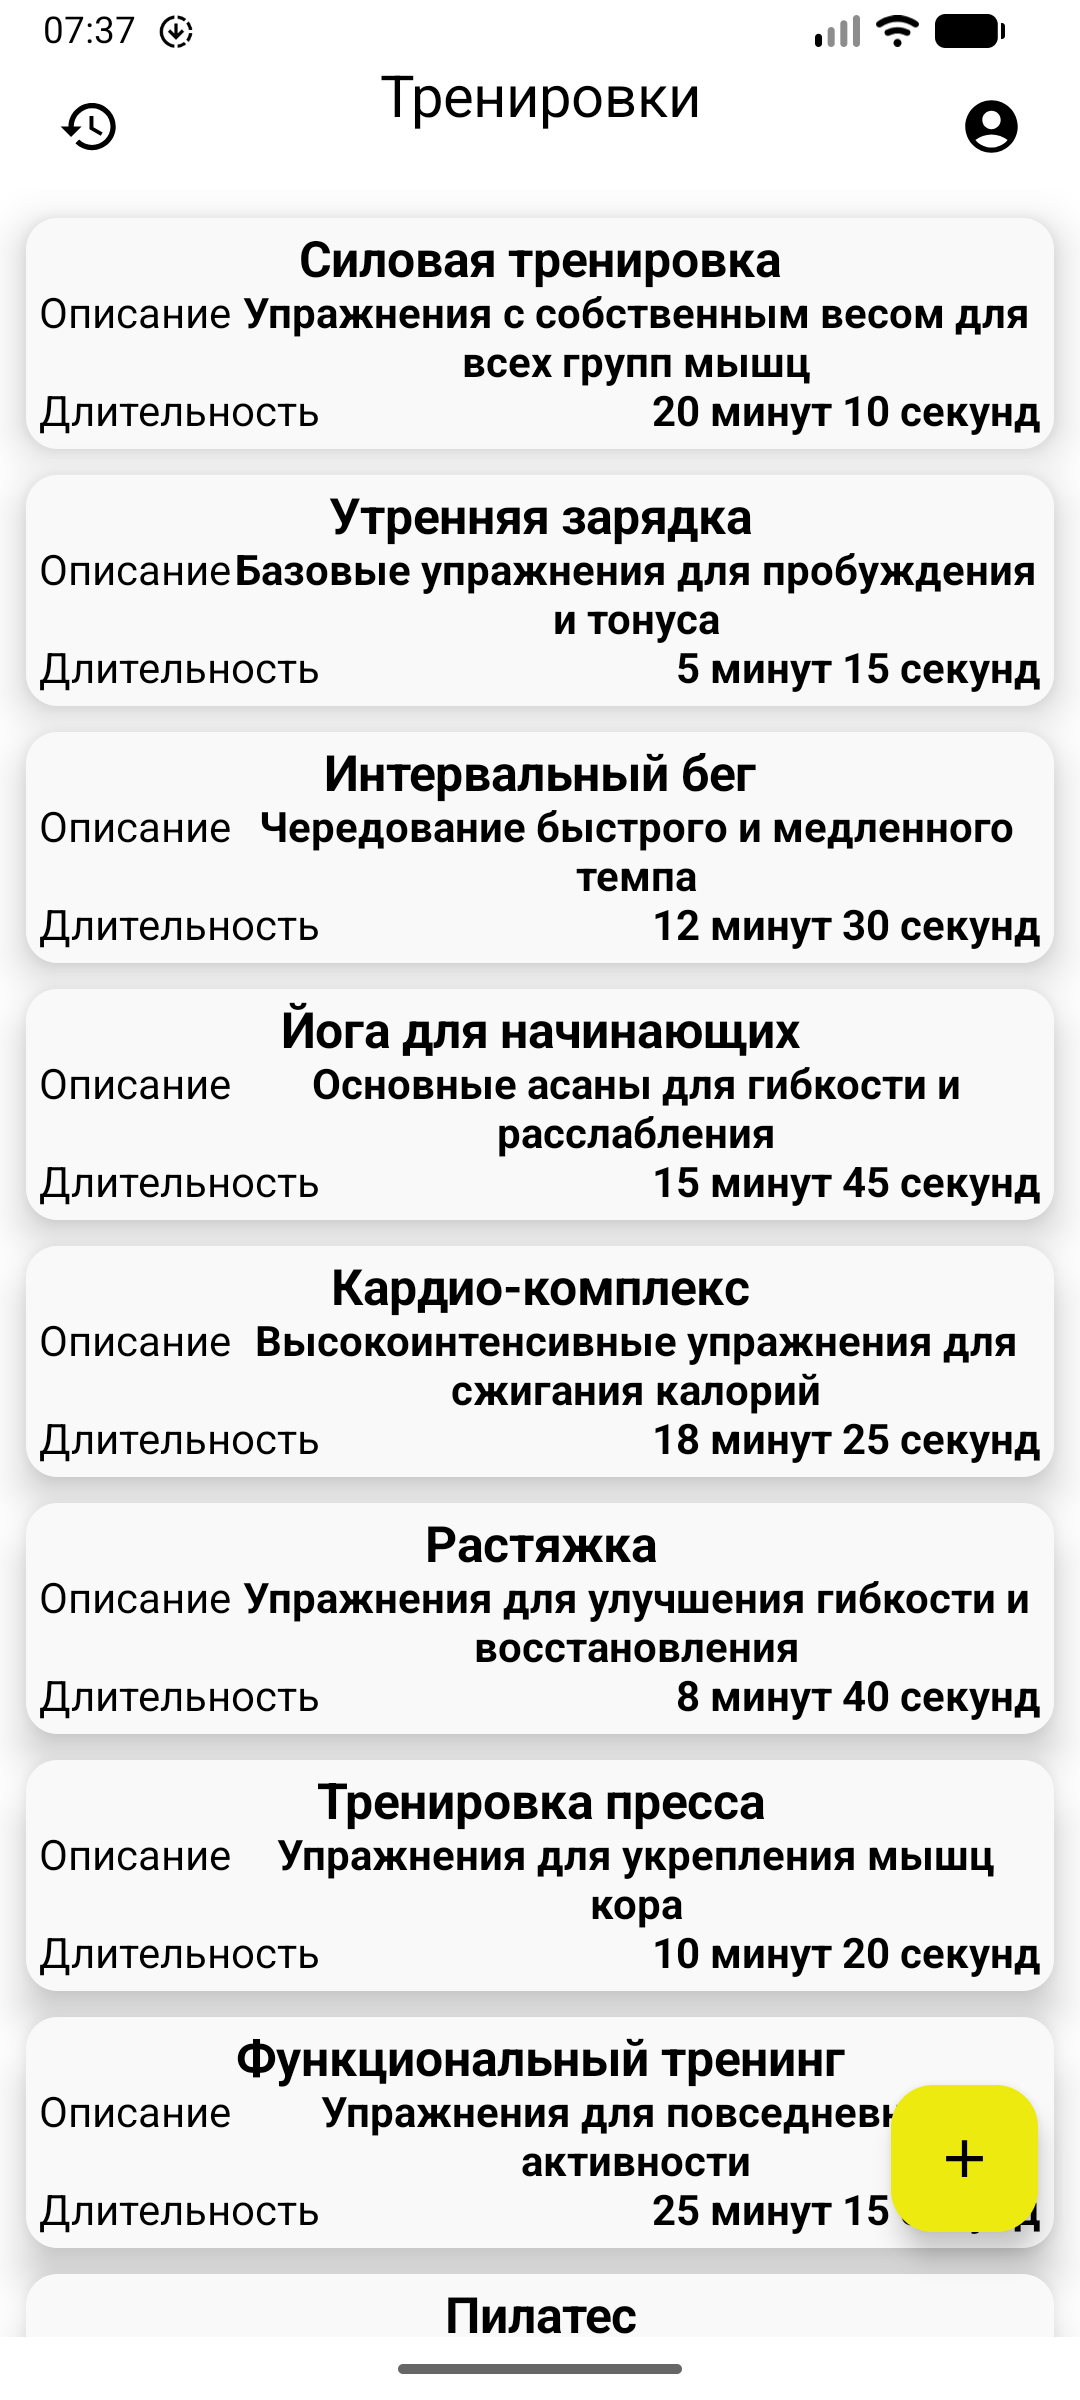
\includegraphics[width=\linewidth]{images/android_screens/main_screen.png}
        \captionof{figure}{Главный экран}
        \label{fig:main}
    \end{minipage}\hfill
    \begin{minipage}{0.18\textwidth}
        \centering
        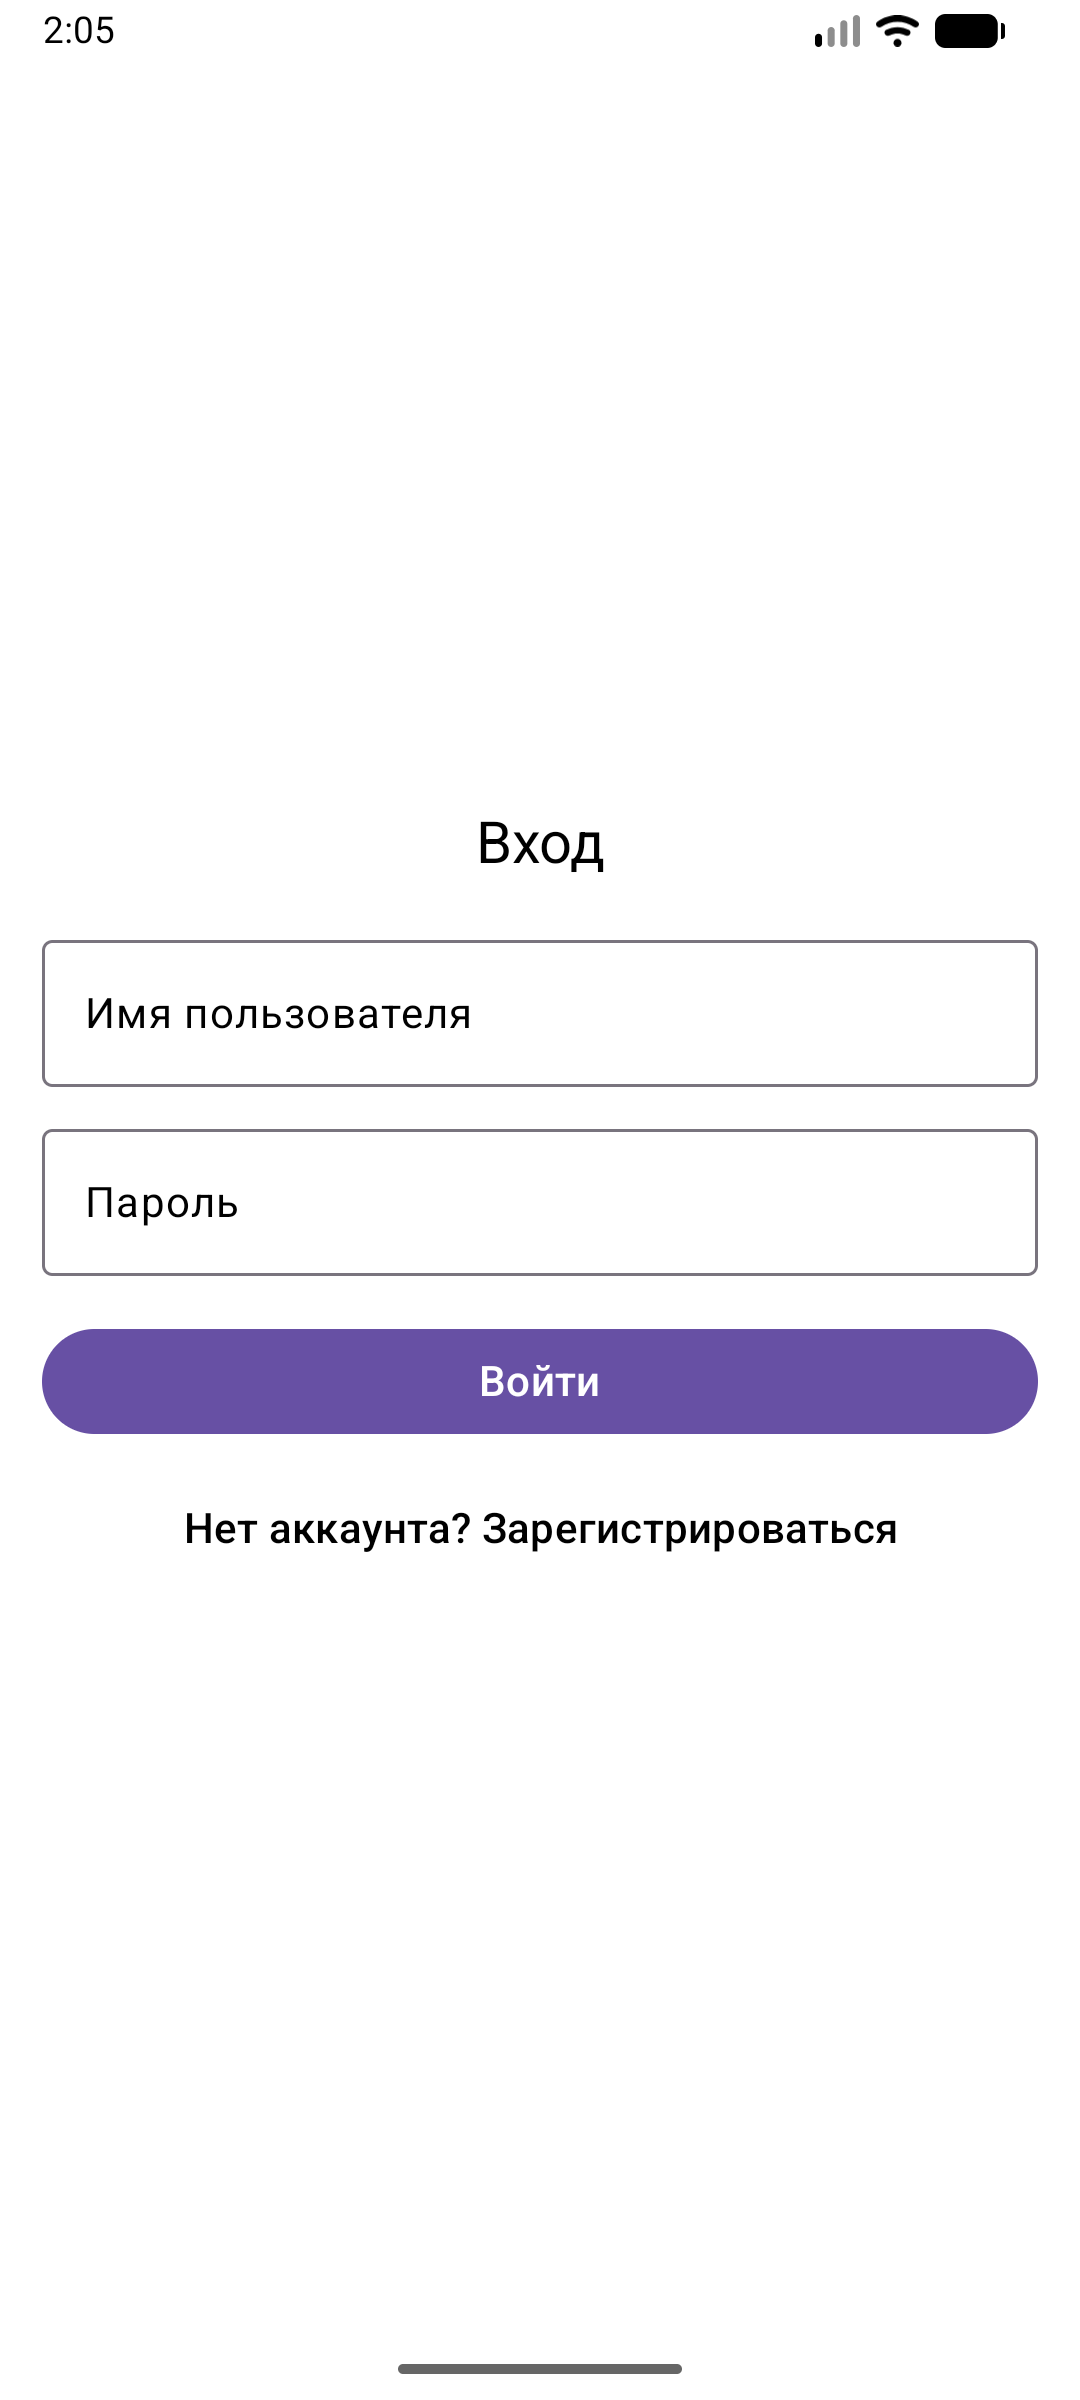
\includegraphics[width=\linewidth]{images/android_screens/sign_in.png}
        \captionof{figure}{Вход}
        \label{fig:signin}
    \end{minipage}\hfill
    \begin{minipage}{0.18\textwidth}
        \centering
        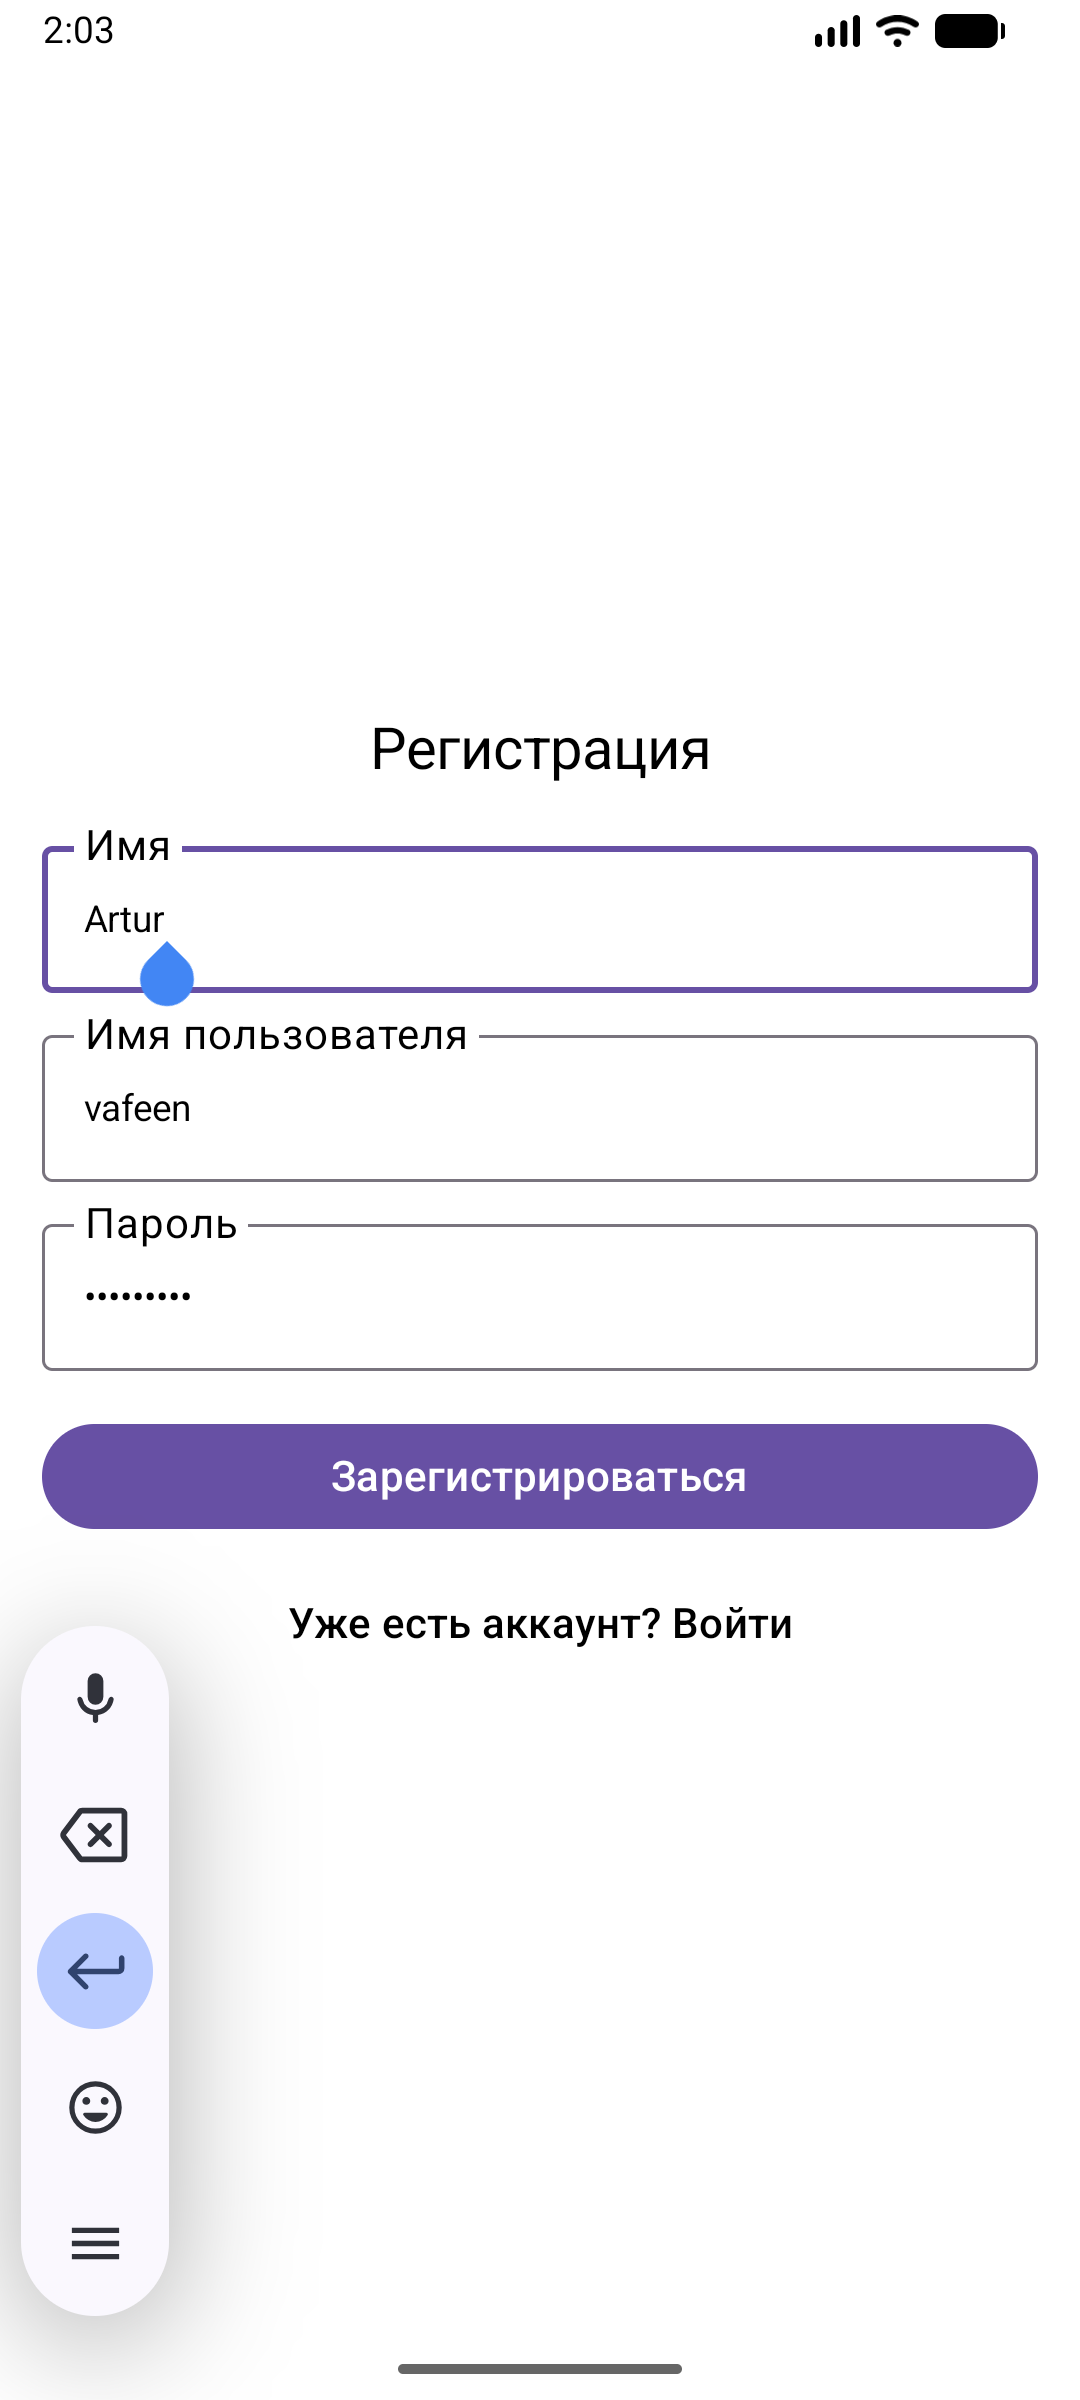
\includegraphics[width=\linewidth]{images/android_screens/sign_up.png}
        \captionof{figure}{Регистрация}
        \label{fig:signup}
    \end{minipage}\hfill
    \begin{minipage}{0.18\textwidth}
        \centering
        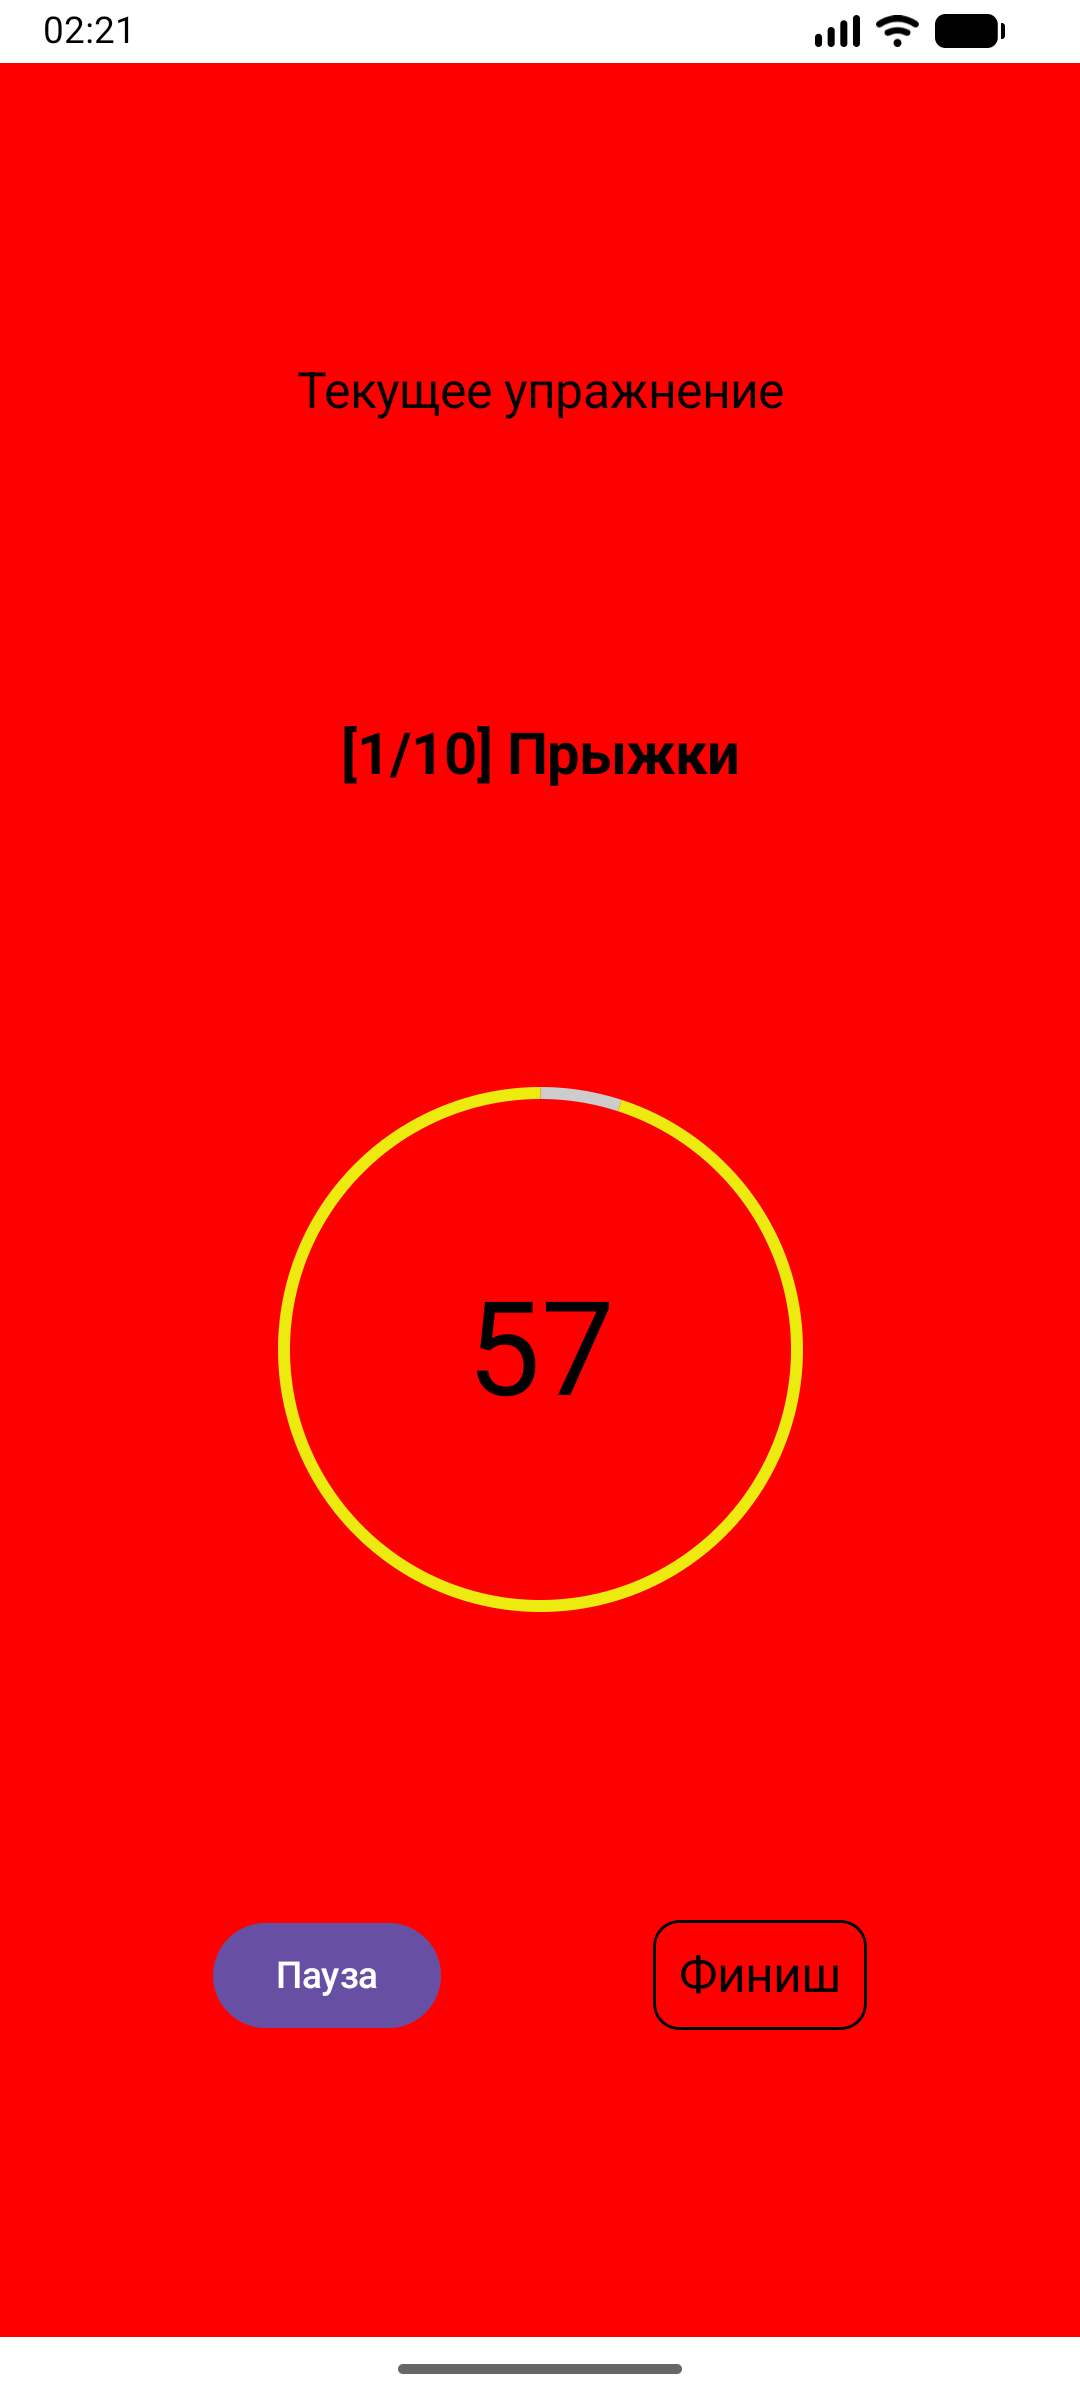
\includegraphics[width=\linewidth]{images/android_screens/training.png}
        \captionof{figure}{Тренировка}
        \label{fig:training}
    \end{minipage}\hfill
    \begin{minipage}{0.18\textwidth}
        \centering
        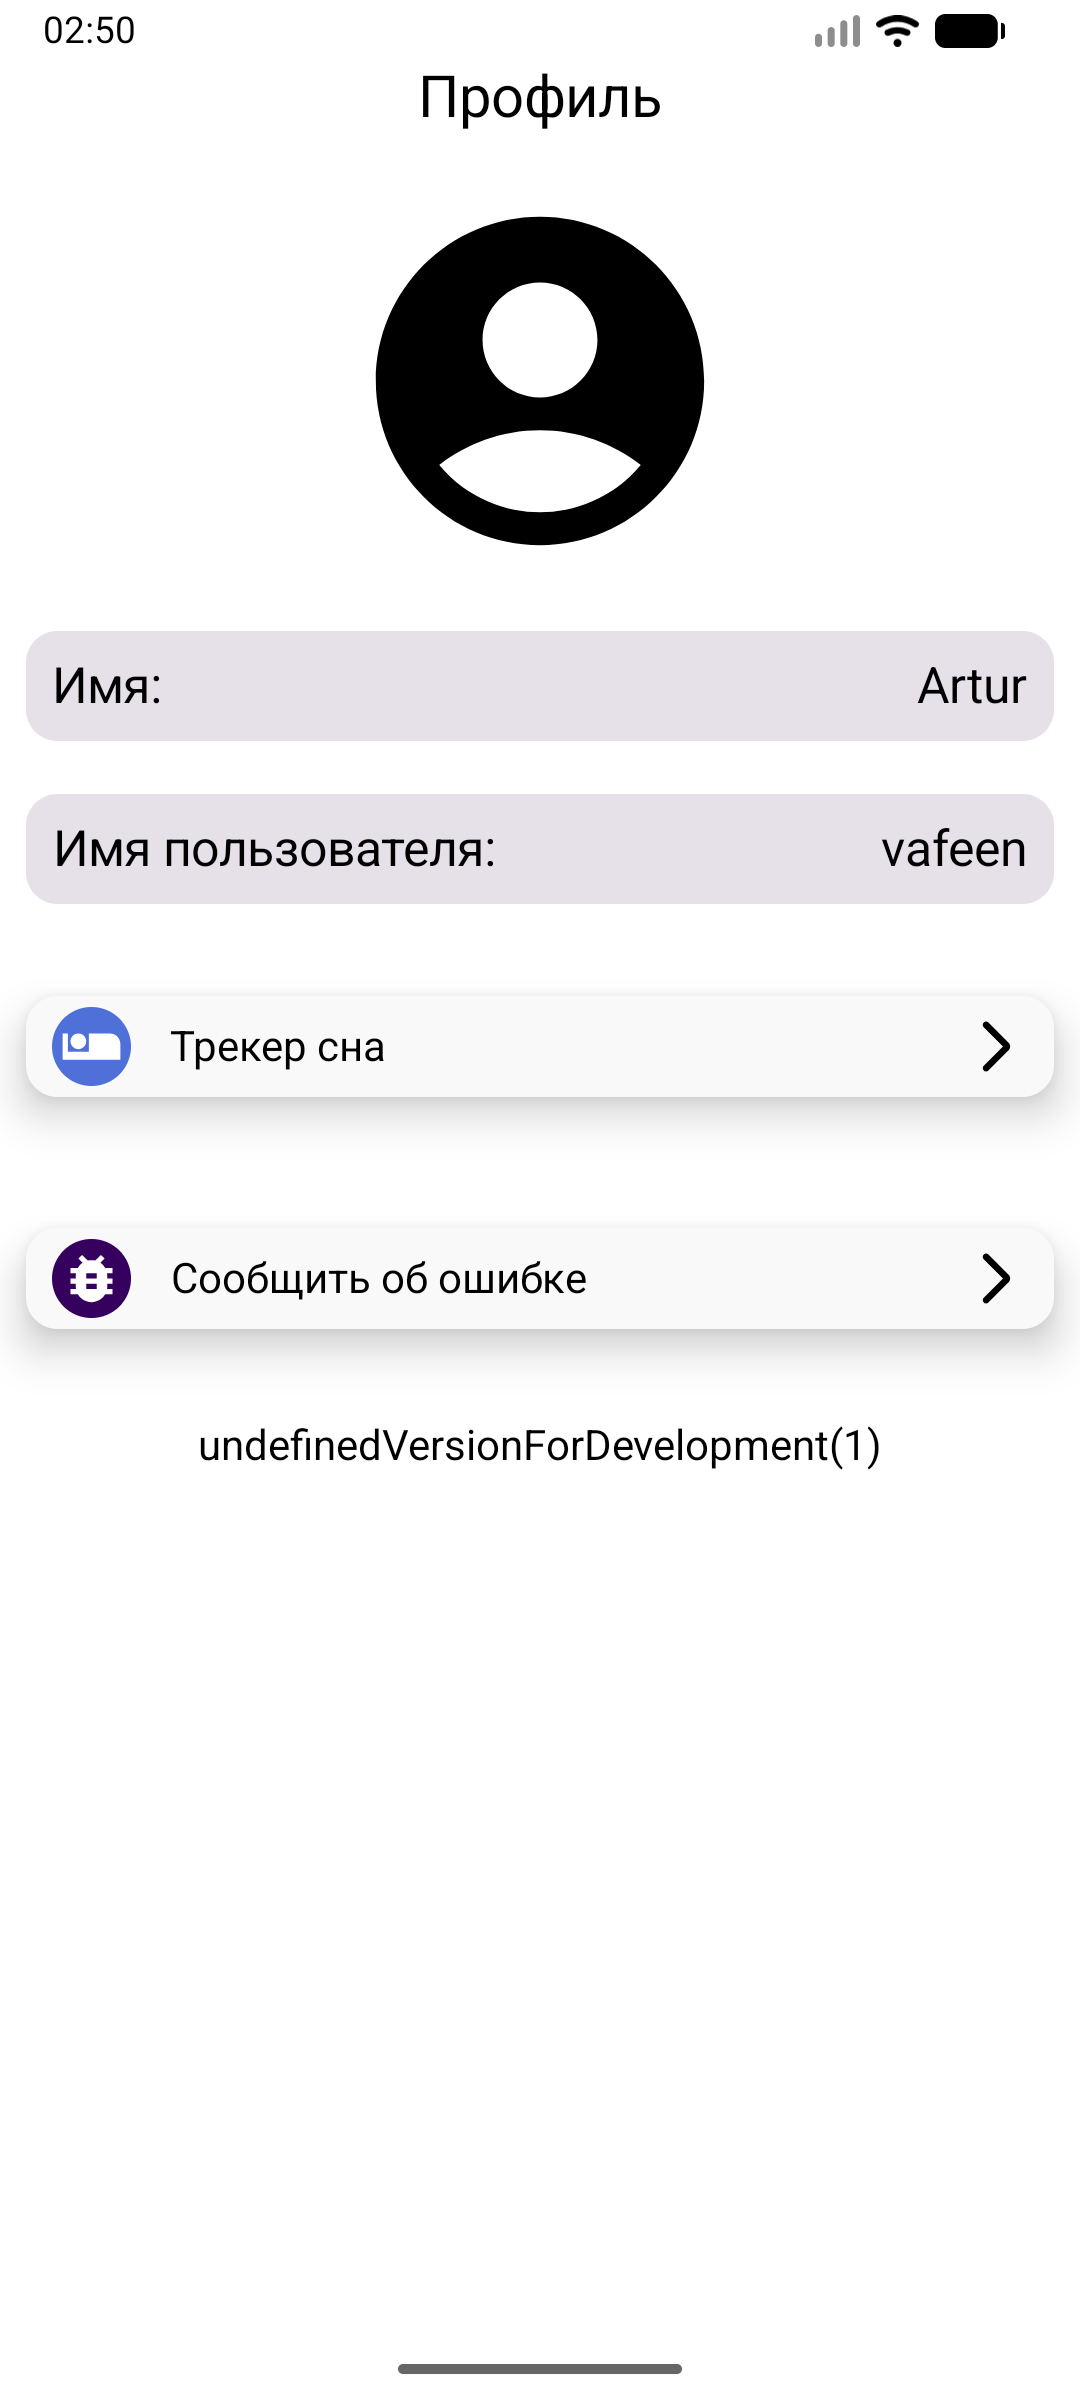
\includegraphics[width=\linewidth]{images/android_screens/profile_screen.png}
        \captionof{figure}{Профиль}
        \label{fig:profile}
    \end{minipage}
    \caption*{}
\end{figure}

\begin{figure}[htbp]
    \centering
    \begin{minipage}{0.18\textwidth}
        \centering
        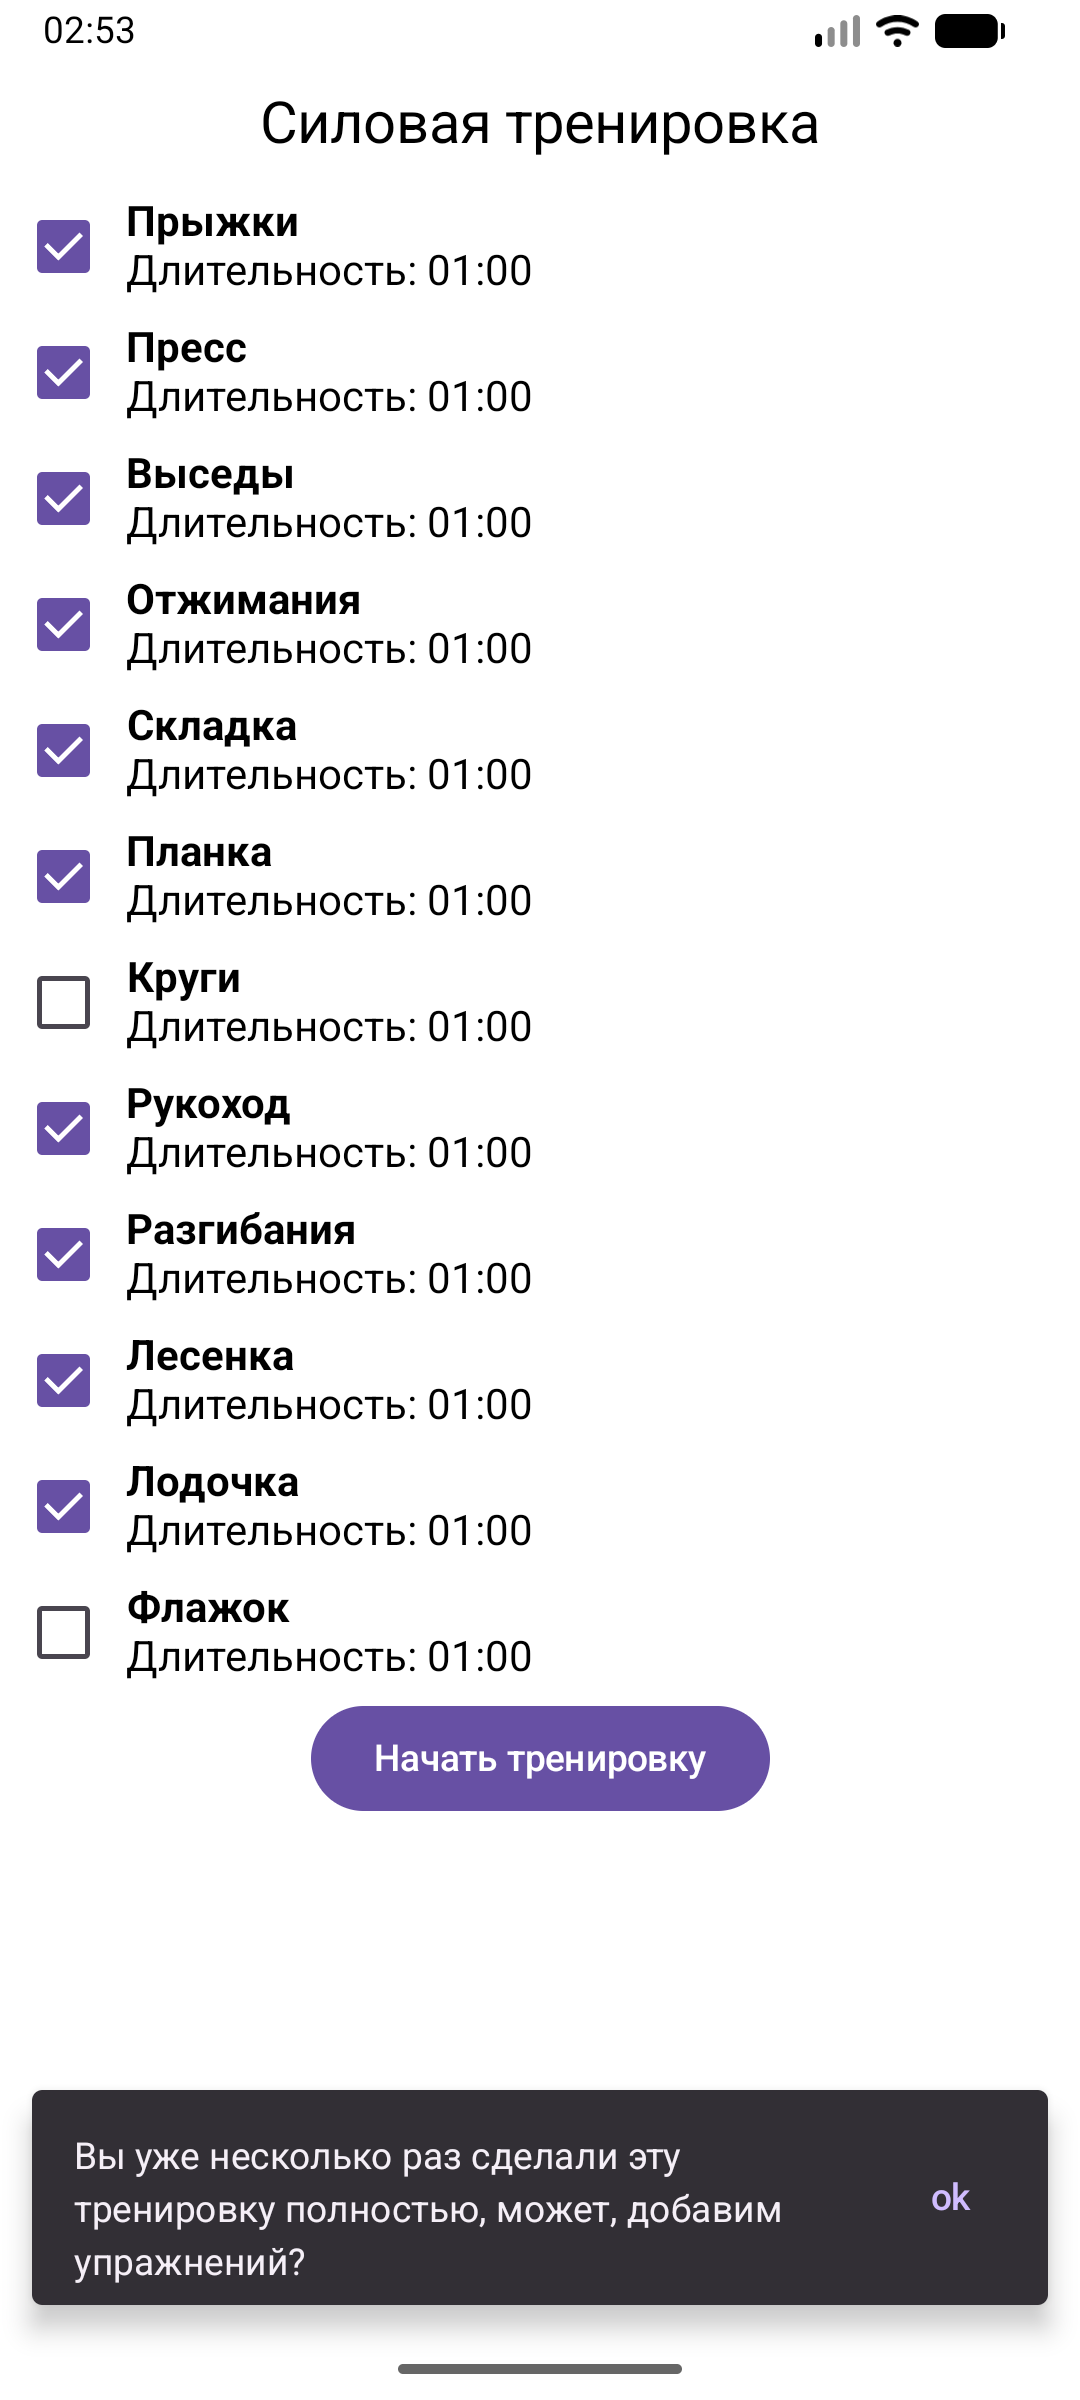
\includegraphics[width=\linewidth]{images/android_screens/before_training.png}
        \captionof{figure}{Перед тренировкой}
        \label{fig:before}
    \end{minipage}\hfill
    \begin{minipage}{0.18\textwidth}
        \centering
        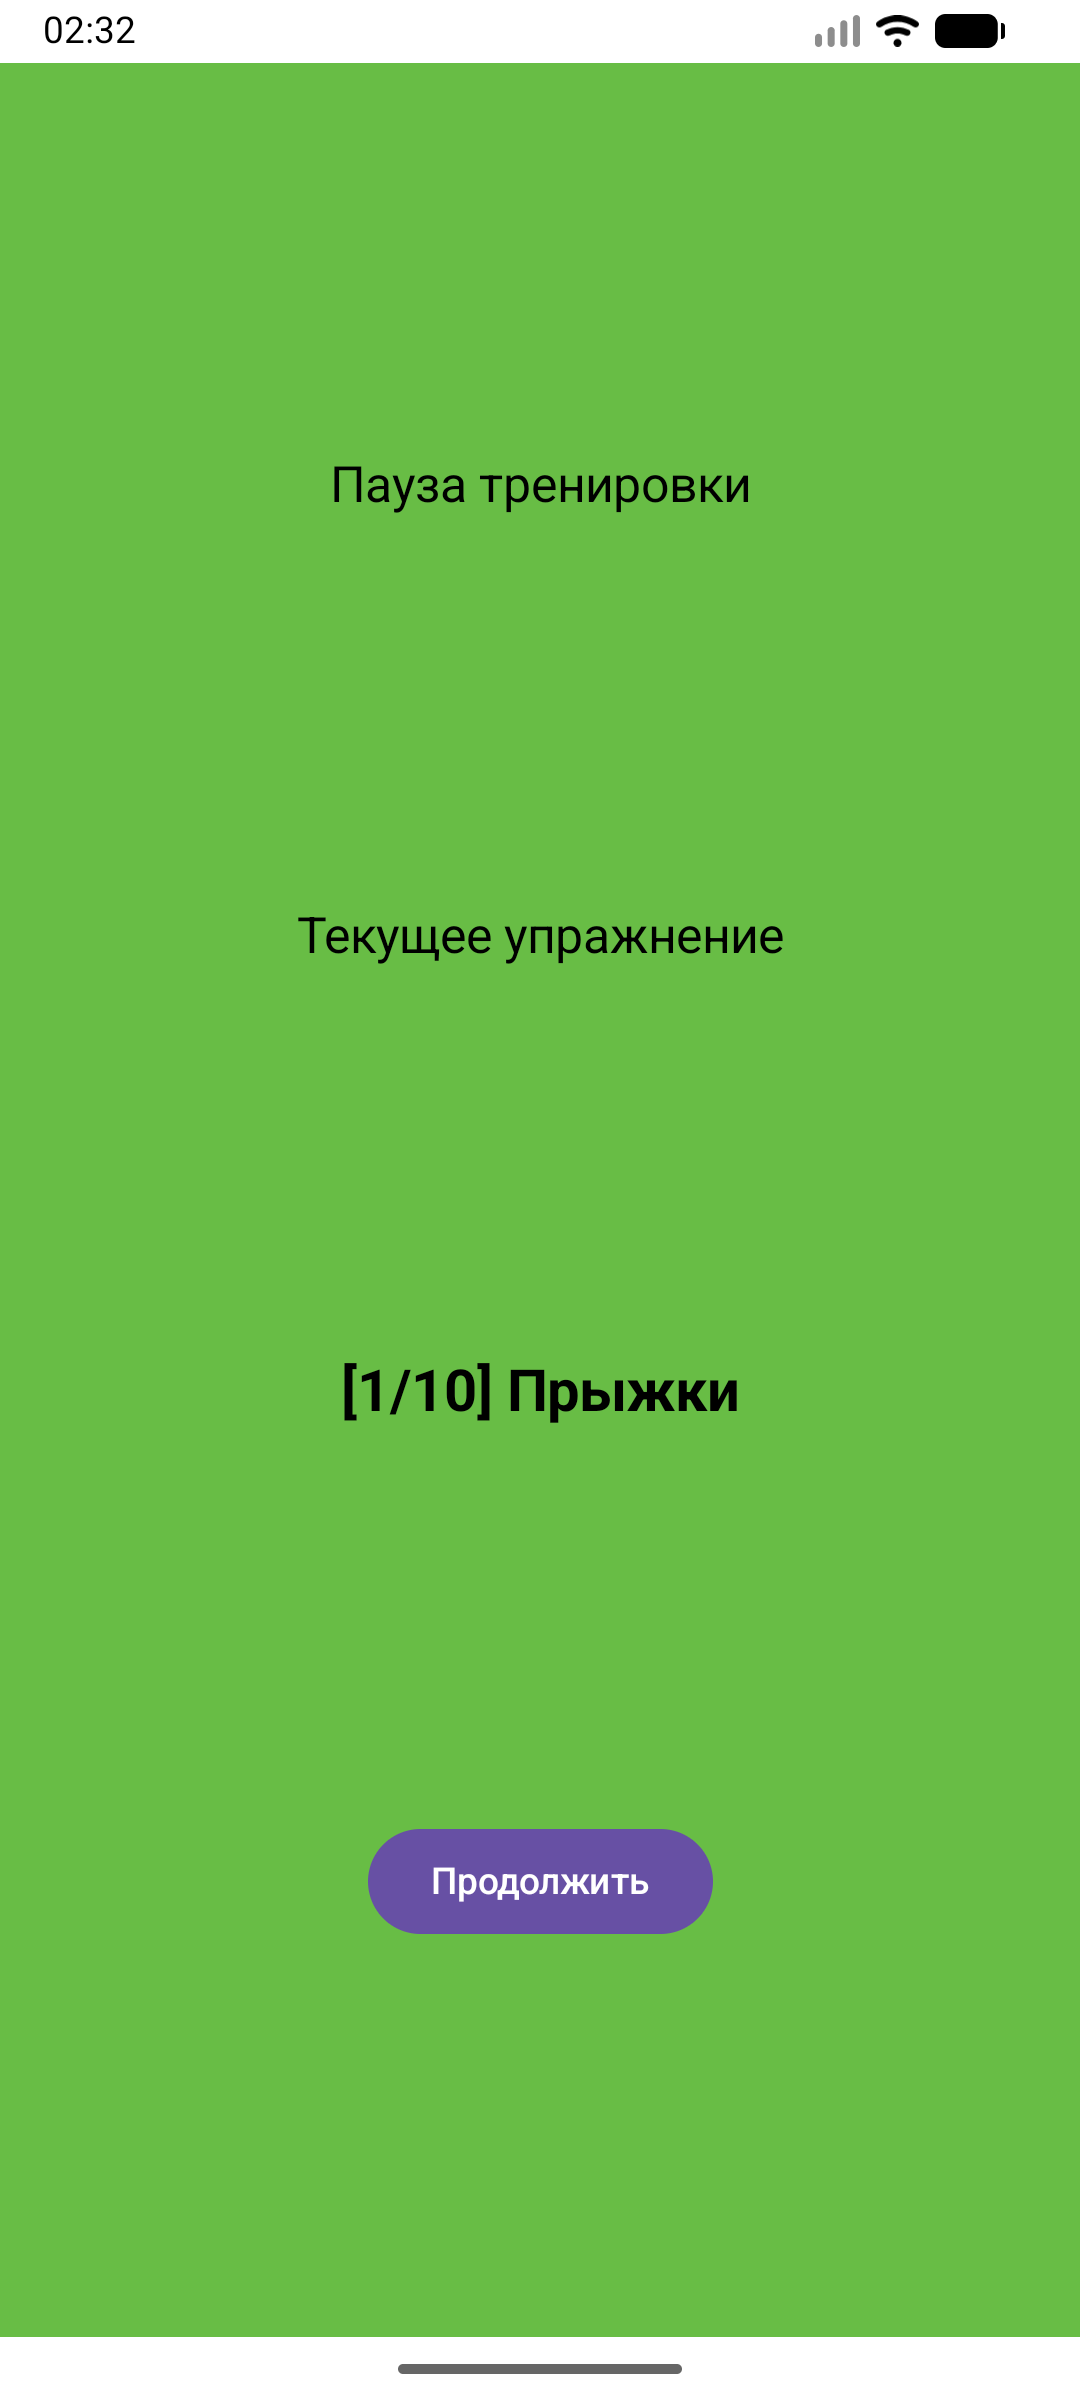
\includegraphics[width=\linewidth]{images/android_screens/pause.png}
        \captionof{figure}{Пауза}
        \label{fig:pause}
    \end{minipage}\hfill
    \begin{minipage}{0.18\textwidth}
        \centering
        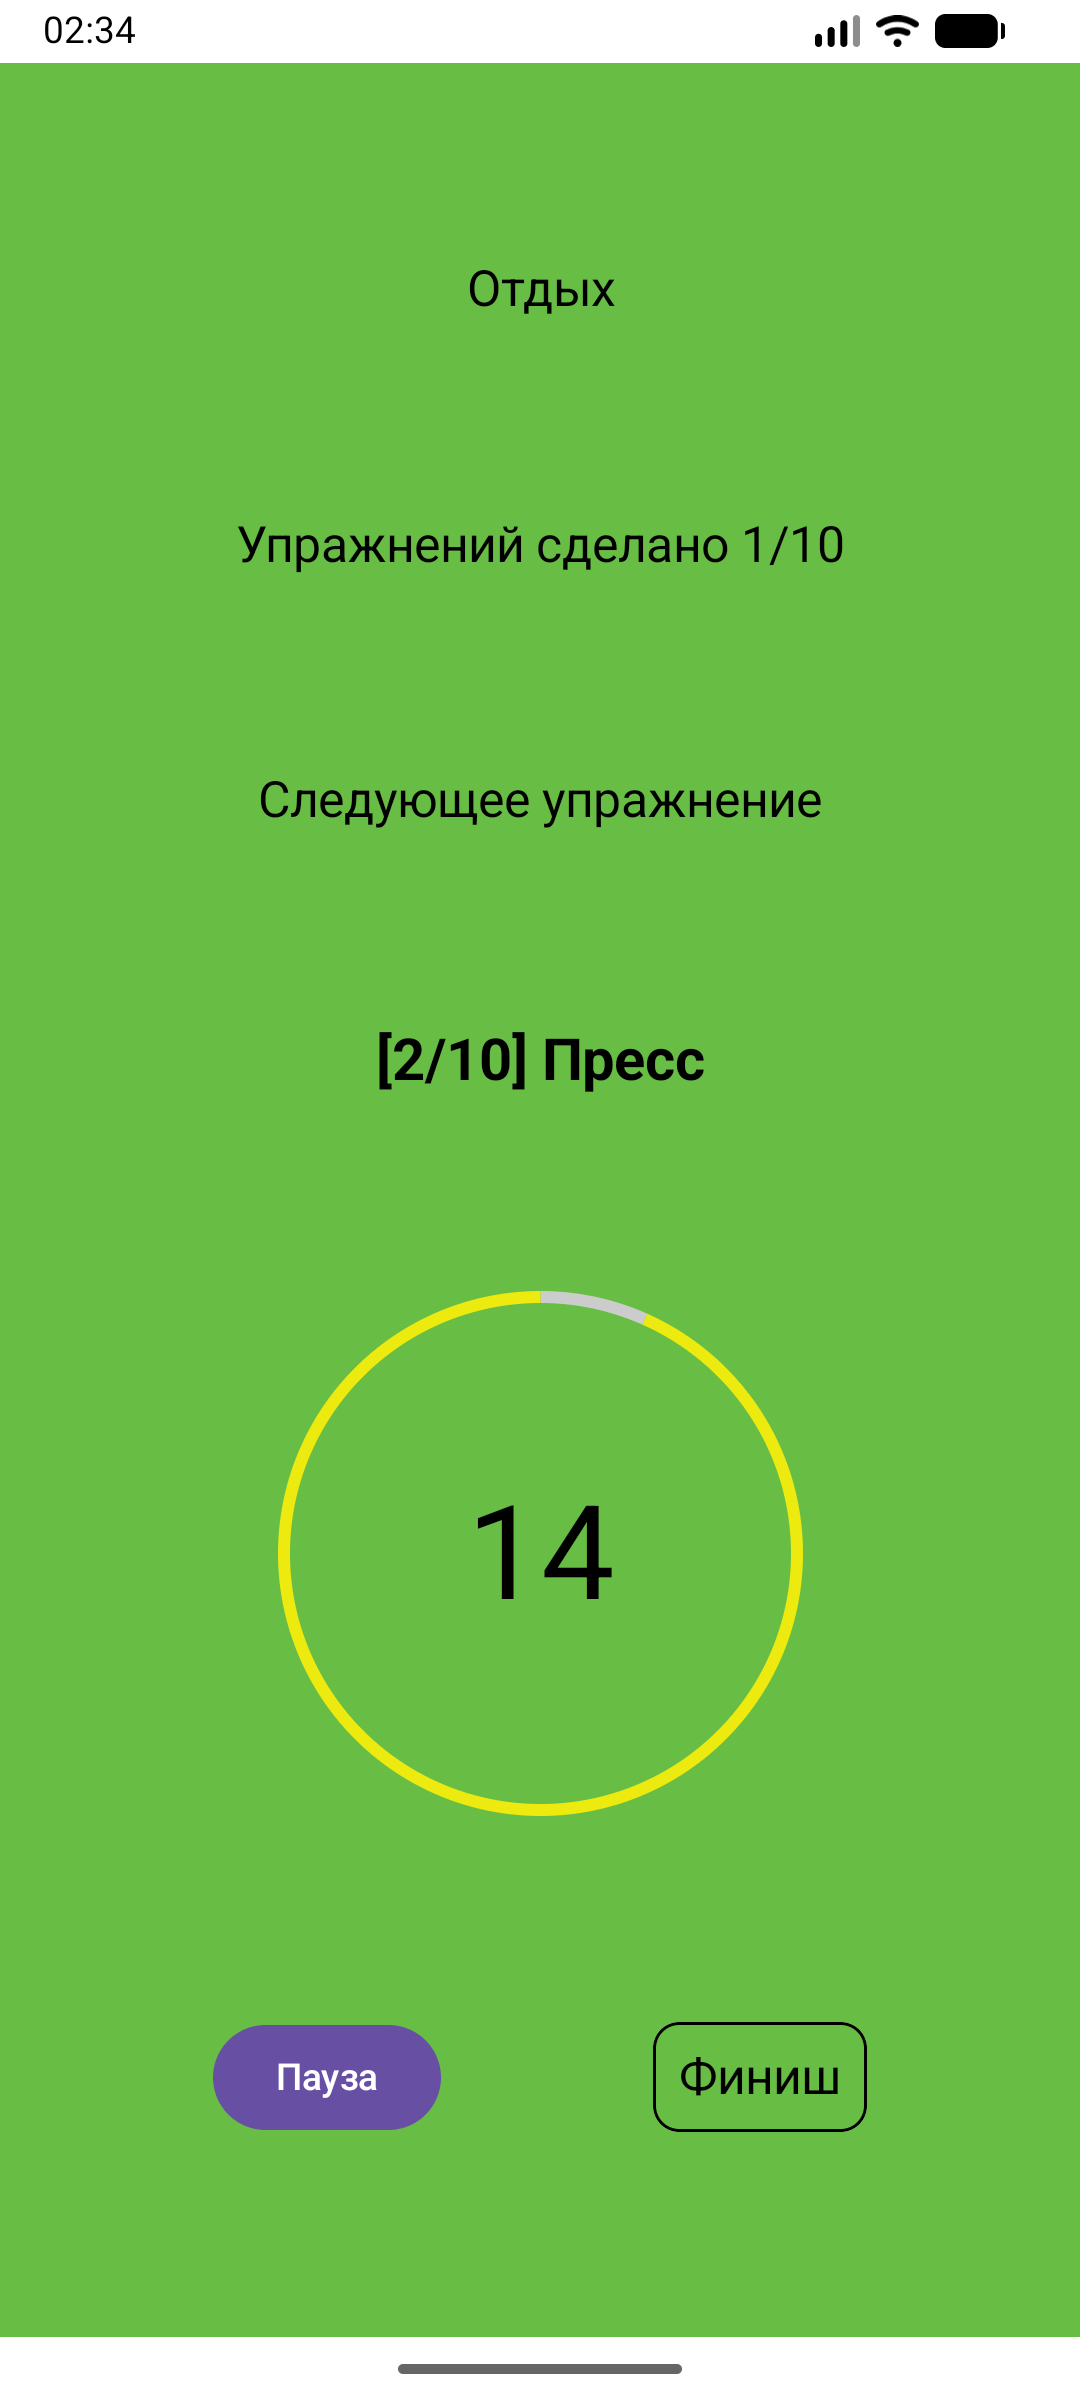
\includegraphics[width=\linewidth]{images/android_screens/rest.png}
        \captionof{figure}{Отдых}
        \label{fig:rest}
    \end{minipage}\hfill
    \begin{minipage}{0.18\textwidth}
        \centering
        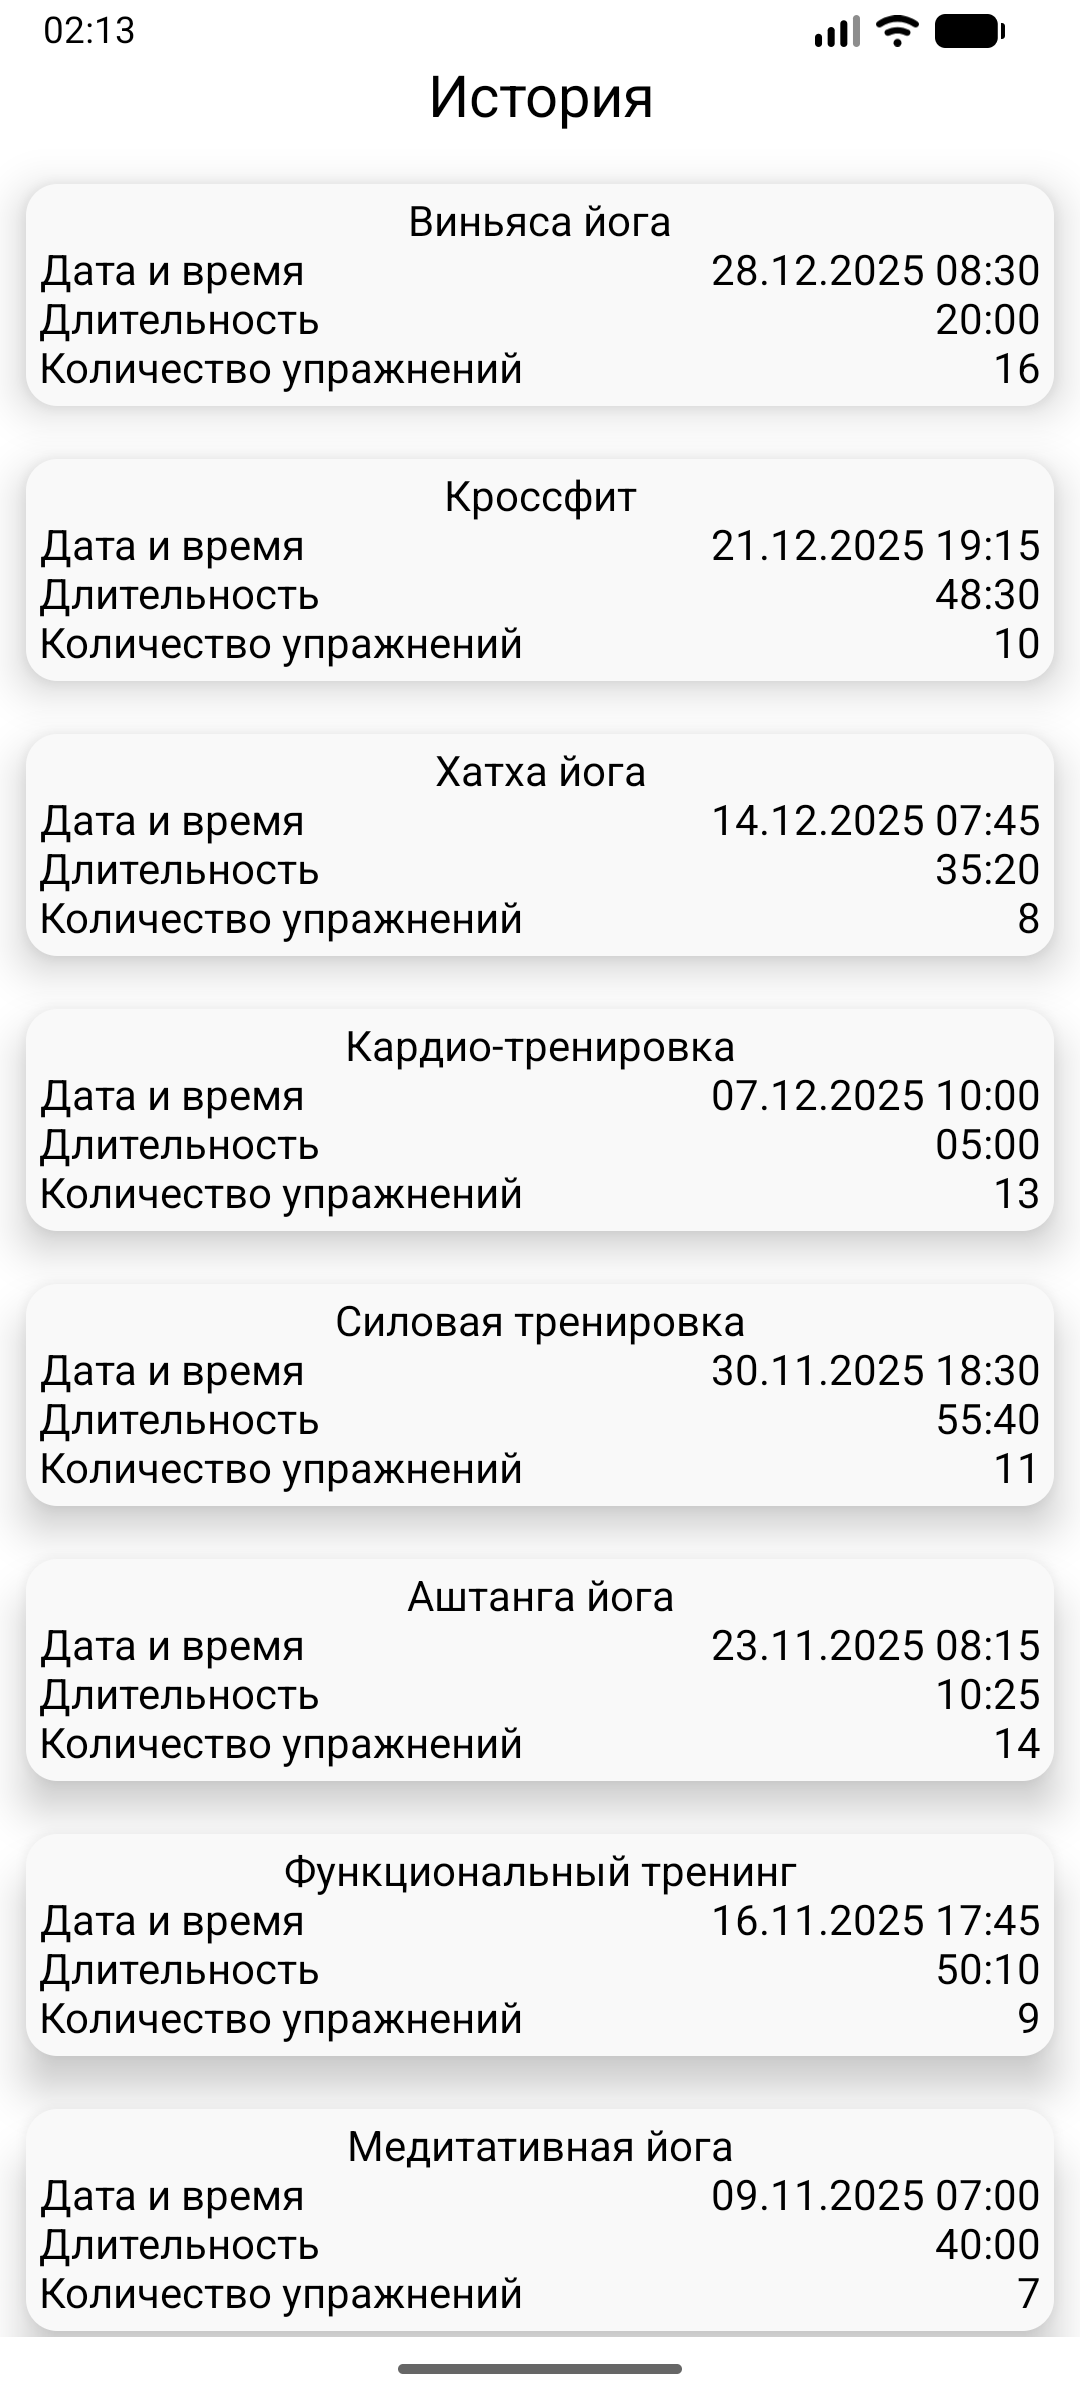
\includegraphics[width=\linewidth]{images/android_screens/history_screen.png}
        \captionof{figure}{История}
        \label{fig:history}
    \end{minipage}\hfill
    \begin{minipage}{0.18\textwidth}
        \centering
        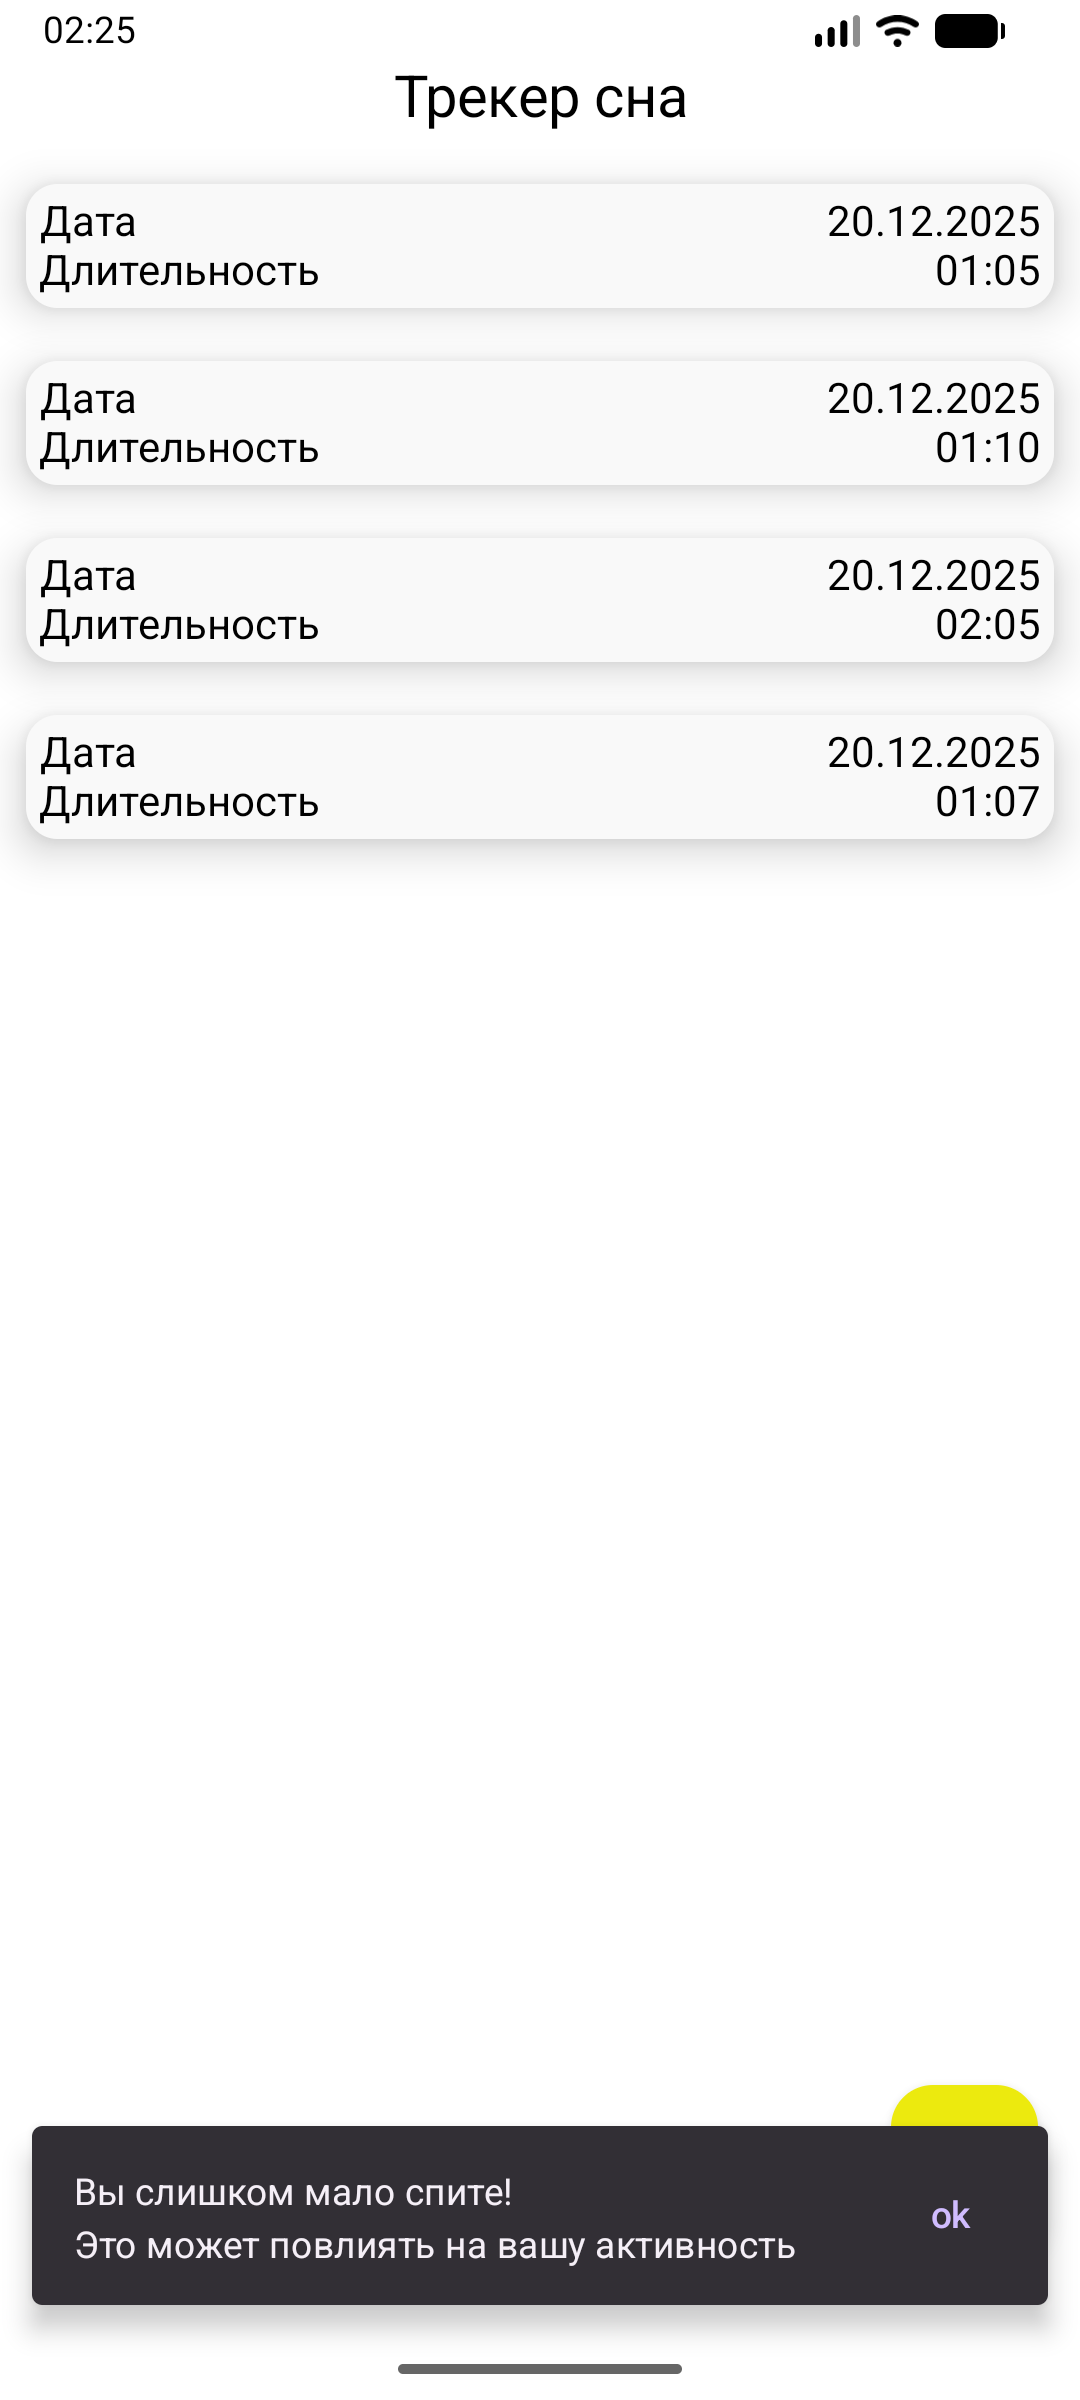
\includegraphics[width=\linewidth]{images/android_screens/sleep_tracker.png}
        \captionof{figure}{Трекер сна}
        \label{fig:sleep}
    \end{minipage}
    \caption*{}
\end{figure}

\subsection{Реализация навигации}

На данном этапе связаны все свёрстанные экраны в единое приложение. Навигация реализована с использованием Jetpack Navigation Component, интегрированного с Jetpack Compose. В приложении применён подход single activity — все экраны представляют собой composable-функции, а управление переходами осуществляется через NavHost и NavController.

Главным контейнером навигации является MainActivity, которая через \texttt{setContent} разворачивает NavHost. В файле навигационного графа определены все возможные маршруты (routes) приложения:
\begin{itemize}
    \item \texttt{auth} — экран входа/регистрации;
    \item \texttt{main} — главный экран со списком тренировок;
    \item \texttt{training/\{workoutId\}} — экран проведения тренировки (с параметром идентификатора);
    \item \texttt{sleep\_tracker} — экран трекера сна;
    \item \texttt{history} — экран истории тренировок;
    \item \texttt{profile} — экран профиля пользователя;
    \item \texttt{before\_training/\{workoutId\}} — экран подготовки к тренировке (выбор упражнений).
\end{itemize}

Для каждого маршрута указана composable-функция, которая отображается при переходе. Стартовым экраном является \texttt{auth} (если пользователь не авторизован) или \texttt{main} (если токен уже сохранён). Для проверки состояния аутентификации используется NavController вместе с условной логикой: при успешном входе выполняется \texttt{navController.navigate("main")} с очисткой back stack (\texttt{popUpTo("auth") \{inclusive = true\}}).

Переходы между экранами инициируются вызовами \texttt{navController.navigate(route)}. Например, на главном экране при нажатии на тренировку вызывается \texttt{navController.navigate("before\_training/\$workoutId")}. После завершения тренировки или подготовки выполняется возврат на предыдущий экран через \texttt{navController.popBackStack()}. Для передачи данных между экранами используются аргументы маршрута (например, \texttt{workoutId}) или \texttt{SavedStateHandle} в ViewModel.

Анимации переходов реализованы через параметры \texttt{enterTransition} и \texttt{exitTransition} в вызове \texttt{composable} (например, \texttt{fadeIn() + slideInHorizontally()}). Back-стек управляется автоматически NavController: последовательные экраны складываются в стек, и кнопка «Назад» (системная или в приложении) возвращает пользователя на предыдущий экран. Для кнопки «Назад» в верхнем тулбаре используется \texttt{BackHandler} или стандартная кнопка, вызывающая \texttt{navController.popBackStack()}.

Благодаря использованию Navigation Component код навигации остаётся декларативным, типобезопасным и легко поддерживаемым.

\subsection{Сущности базы данных}

На данном этапе определены Entity-классы, описывающие таблицы базы данных. На рис.~\ref{fig:db_schema} представлена схема базы данных, показывающая связи между таблицами.

\begin{figure}[H]
    \centering
    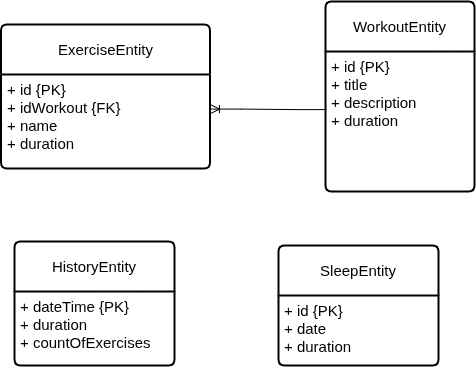
\includegraphics[width=1\textwidth]{images/diagrams/Схема бд.png}
    \caption{Схема базы данных}
    \label{fig:db_schema}
\end{figure}

Entity-классы:
\begin{itemize}
    \item \texttt{ExerciseEntity} — содержит поля: идентификатор упражнения, идентификатор тренировки, название, продолжительность.
    \item \texttt{WorkoutEntity} — содержит идентификатор, заголовок, описание, общую длительность.
    \item \texttt{SleepEntity} — содержит идентификатор, дату, продолжительность сна в минутах.
    \item \texttt{HistoryEntity} — содержит дату и время тренировки, длительность, количество выполненных упражнений.
\end{itemize}
Связи между таблицами (например, «тренировка — упражнения») обрабатываются в репозиториях с помощью нескольких запросов.



\subsection{Реализация серверного приложения}

Серверная часть реализована на Kotlin с использованием фреймворка Ktor. В качестве базы данных для хранения пользователей, тренировок и записей о сне используется PostgreSQL. API построено по принципу REST и поддерживает следующие эндпоинты:

\begin{itemize}
    \item \texttt{POST /register} — регистрация нового пользователя (принимает JSON с полями \texttt{username}, \texttt{password}, \texttt{name}, возвращает сообщение об успехе);
    \item \texttt{POST /login} — аутентификация (принимает \texttt{username}, \texttt{password}, возвращает JWT-токен);
    \item \texttt{GET /sleep} — получение всех записей о сне текущего пользователя (требует JWT);
    \item \texttt{POST /sleep} — добавление новой записи о сне (принимает \texttt{date}, \texttt{duration}, возвращает созданную запись с \texttt{id});
    \item \texttt{PUT /sleep/\{id\}} — обновление записи о сне по \texttt{id} (принимает обновлённые поля, возвращает сообщение об успехе);
    \item \texttt{DELETE /sleep/\{id\}} — удаление записи о сне по \texttt{id};
    \item \texttt{GET /exercises} — получение списка всех упражнений;
    \item \texttt{POST /exercises} — добавление нового упражнения (принимает \texttt{name}, \texttt{isIncludedToTraining}, \texttt{duration});
    \item \texttt{GET /workouts} — получение всех тренировок с детальным списком упражнений;
    \item \texttt{POST /workouts} — создание новой тренировки (принимает \texttt{dateTime}, \texttt{duration}, список \texttt{exercises});
    \item \texttt{DELETE /workouts/\{dateTime\}} — удаление тренировки по её дате-времени.
\end{itemize}

Все эндпоинты, кроме \texttt{/register} и \texttt{/login}, защищены middleware, проверяющим JWT-токен (передаётся в заголовке \texttt{Authorization: Bearer <token>}). 

Структура хранения данных серверного приложения отражена на рис.~\ref{fig:server_db_schema}.

Entity-классы:

\begin{itemize}
\item UserDataEntity — содержит поля: идентификатор, логин, имя, хэш пароля.

\item ExerciseEntity — содержит поля: идентификатор, идентификатор пользователя, идентификатор тренировки, название, продолжительность.

\item WorkoutEntity — содержит поля: идентификатор, идентификатор пользователя, заголовок, описание, продолжительность.

\item SleepEntity — содержит поля: идентификатор, идентификатор пользователя, дата, продолжительность (в минутах).
(Составной первичный ключ: идентификатор + идентификатор пользователя.)

\item HistoryEntity — содержит поля: идентификатор пользователя, дата и время, продолжительность, количество упражнений.
(Составной первичный ключ: идентификатор пользователя + дата и время.)
\end{itemize}

\begin{figure}[h]
    \centering
    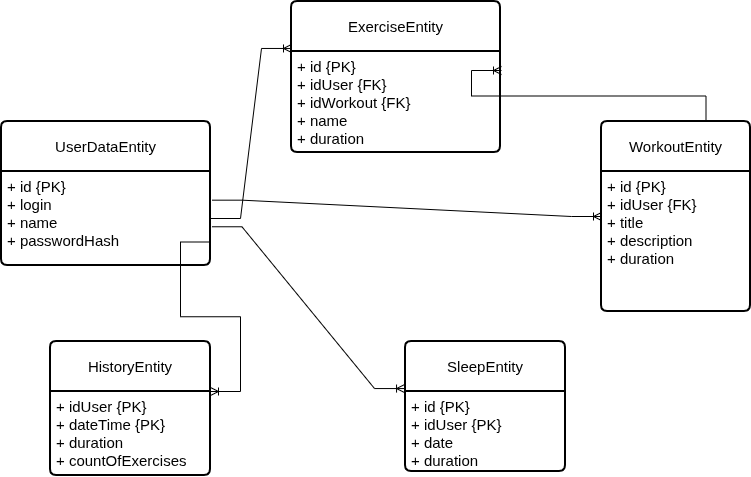
\includegraphics[width=0.8\textwidth]{images/diagrams/Схема бд бэкенд.png}
    \caption{Схема базы данных серверного приложения}
    \label{fig:server_db_schema}
\end{figure}

Сервер развёрнут на облачной платформе и доступен по HTTPS.

\subsection{Проверка HTTP-запросов к серверному приложению}

Для тестирования API использовался инструмент Postman. Были проверены все перечисленные эндпоинты. Ниже перечислены ключевые проверки:

\begin{itemize}
    \item \texttt{POST /register} — отправка JSON с \texttt{username}, \texttt{password}, \texttt{name}; получен ответ с кодом 201 и сообщением \texttt{"User registered successfully"}.
    \item \texttt{POST /login} — отправка \texttt{username}/\texttt{password}; получен \texttt{accessToken} (JWT).
    \item \texttt{GET /sleep} — с токеном в заголовке \texttt{Authorization}; получен массив записей сна (даже пустой).
    \item \texttt{POST /sleep} — отправка \texttt{date} и \texttt{duration}; получен ответ с \texttt{id} созданной записи.
    \item \texttt{PUT /sleep/\{id\}} — обновление существующей записи; получен ответ с подтверждением.
    \item \texttt{DELETE /sleep/\{id\}} — удаление записи; ответ \texttt{"Sleep record deleted"}.
    \item \texttt{GET /exercises} — получен список упражнений.
    \item \texttt{POST /exercises} — добавление нового упражнения; возвращён \texttt{id}.
    \item \texttt{GET /workouts} — получен массив тренировок, каждая из которых содержит вложенный массив упражнений.
    \item \texttt{POST /workouts} — отправка \texttt{dateTime}, \texttt{duration} и списка \texttt{exercises}; получено подтверждение.
    \item \texttt{DELETE /workouts/\{dateTime\}} — удаление тренировки по дате-времени; ответ \texttt{"Workout deleted"}.
\end{itemize}

Все запросы успешно выполнялись, возвращая ожидаемые коды состояния (200, 201, 204) и корректные JSON-данные. Ошибки (неверный токен, отсутствие соединения, невалидные данные) обрабатываются и возвращают соответствующие коды 401, 400, 404. Результаты запросов показаны в приложении 2.

\subsection{Получение OpenSSL-сертификата для защищённого соединения}

Для обеспечения безопасной передачи данных между клиентом и сервером было настроено HTTPS-соединение. Самоподписанный сертификат сгенерирован с помощью OpenSSL:
\begin{verbatim}
openssl req -x509 -newkey rsa:4096 -keyout key.pem -out cert.pem -days 365 -nodes
\end{verbatim}
Полученные файлы \texttt{cert.pem} и \texttt{key.pem} были размещены на сервере, а в коде серверного приложения добавлена конфигурация HTTPS:
\begin{verbatim}
const https = require('https');
const options = { key: fs.readFileSync('key.pem'), cert: fs.readFileSync('cert.pem') };
https.createServer(options, app).listen(443);
\end{verbatim}
В клиентском приложении Retrofit настроен на работу с HTTPS-URL, проверка сертификата доверена (для самоподписанного сертификата используется специальный доверенный клиент).

\subsection{Реализация синхронизации с сервером}

Основная цель работы с сетью — взаимодействие с серверным API для авторизации, синхронизации тренировок и данных о сне. На рис.~\ref{fig:network_repos} представлена диаграмма классов для сетевых репозиториев.


\subsubsection{Общая организация сетевого слоя}

Сетевой слой построен на связке Retrofit + OkHttp. В модуле Koin (сетевой модуль) определены:
\begin{itemize}
    \item экземпляр \texttt{OkHttpClient} с интерцепторами для добавления JWT-токена и логирования;
    \item экземпляр \texttt{Retrofit} с базовым URL и конвертером Gson;
    \item реализации интерфейсов удалённых репозиториев.
\end{itemize}

Каждый удалённый репозиторий получает через конструктор соответствующий Retrofit-сервис (интерфейс с аннотациями). Сервисы генерируются автоматически при сборке.


\subsubsection{Интерфейсы репозиториев для работы с сетью}

Ниже представлен список репозиториев для работы с бэкендом:
\begin{itemize}
    \item \texttt{ExerciseRemoteRepository} — объявляет метод для получения полного списка упражнений;
    \item \texttt{HistoryRemoteRepository} — объявляет метод для получения истории завершённых тренировок;
    \item \texttt{WorkoutRemoteRepository} — объявляет методы для получения всех тренировок, отправки новой тренировки и удаления;
    \item \texttt{SleepRemoteRepository} — объявляет методы для получения всех записей о сне пользователя, добавления новой записи, обновления и удаления;
    \item \texttt{UserDataRemoteRepository} — объявляет методы для регистрации нового пользователя и входа в систему.
\end{itemize}

\begin{figure}[H]
    \centering
    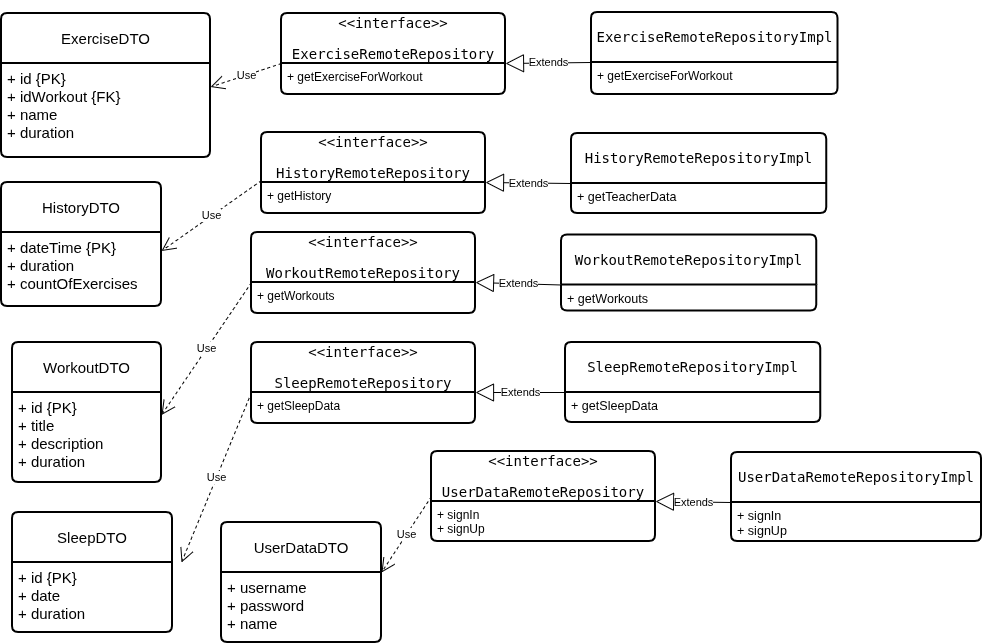
\includegraphics[width=1\textwidth]{images/diagrams/Диаграмма классов сетевых репозиториев.png}
    \caption{Диаграмма классов для сетевых репозиториев}
    \label{fig:network_repos}
\end{figure}

\subsubsection{Реализации интерфейсов репозиториев для работы с сетью}

Каждый класс-реализация удалённого репозитория принимает в конструкторе соответствующий Retrofit-сервис и опционально \texttt{ConnectivityManager} для проверки сети. Методы вызывают suspend-функции сервиса, оборачивают результат в \texttt{Result<T>} (успех или ошибка) и обрабатывают исключения. Ниже приведено описание каждого репозитория.

\begin{itemize}
    \item \texttt{ExerciseRemoteRepositoryImpl} — реализует \texttt{ExerciseRemoteRepository}. В конструктор передаётся \texttt{ExerciseApiService}. Метод \texttt{getExercises()} вызывает \texttt{service.getExercises()}. При успехе возвращает список \texttt{ExerciseDTO}, при ошибке — \texttt{Result.failure}. Не требует проверки соединения, так как сетевые ошибки обрабатываются через исключения Retrofit.

    \item \texttt{HistoryRemoteRepositoryImpl} — реализует \texttt{HistoryRemoteRepository}. Зависит от \texttt{HistoryApiService}. Метод \texttt{getHistory()} вызывает \texttt{service.getHistory()} и возвращает список \texttt{HistoryDTO} или ошибку. Используется для получения истории завершённых тренировок с сервера.

    \item \texttt{WorkoutRemoteRepositoryImpl} — реализует \texttt{WorkoutRemoteRepository}. Принимает \texttt{WorkoutApiService} и \texttt{ConnectivityManager}. Предоставляет три метода:
        \begin{itemize}
            \item \texttt{getWorkouts()} — вызывает \texttt{service.getWorkouts()}, возвращает список \texttt{WorkoutDTO};
            \item \texttt{postWorkout(workoutDTO)} — отправляет новую тренировку через \texttt{service.postWorkout(...)}, возвращает \texttt{WorkoutDTO} с серверным идентификатором;
            \item \texttt{deleteWorkout(workoutId)} — вызывает \texttt{service.deleteWorkout(workoutId)}.
        \end{itemize}
        Перед каждым вызовом проверяется наличие интернет-соединения; при его отсутствии возвращается \texttt{Result.failure(NoInternetException)}.

    \item \texttt{SleepRemoteRepositoryImpl} — реализует \texttt{SleepRemoteRepository}. Зависит от \texttt{SleepApiService} и \texttt{ConnectivityManager}. Содержит методы для полного CRUD:
        \begin{itemize}
            \item \texttt{getSleepRecords()} — получает все записи о сне пользователя (\texttt{List<SleepDTO>});
            \item \texttt{addSleepRecord(sleepDTO)} — добавляет новую запись;
            \item \texttt{updateSleepRecord(id, sleepDTO)} — обновляет существующую;
            \item \texttt{deleteSleepRecord(id)} — удаляет запись.
        \end{itemize}
        Аналогично проверяет наличие сети перед каждым запросом.

    \item \texttt{UserDataRemoteRepositoryImpl} — реализует \texttt{UserDataRemoteRepository}. Принимает \texttt{UserApiService}. Метод \texttt{register(username, password, displayName)} вызывает \texttt{service.register(...)} и возвращает \texttt{UserDTO} с данными пользователя. Метод \texttt{login(username, password)} вызывает \texttt{service.login(...)} и возвращает \texttt{TokenDTO}, содержащий JWT-токен. Ошибки сети и сервера (например, неверные учётные данные) передаются через \texttt{Result.failure}.
\end{itemize}

Во всех реализациях при успешном вызове сервиса возвращается \texttt{Result.success(data)}, при возникновении исключения (IOException, HttpException и т.д.) — \texttt{Result.failure(exception)}. Такой подход позволяет вызывающему коду единообразно обрабатывать как успешные, так и ошибочные сценарии.

\subsubsection{Обработка данных}

Для преобразования объектов передачи данных, полученных из сети, в доменные модели используются мапперы — отдельные функции расширения, расположенные в пакете \texttt{mappers}. Это позволяет изолировать слой данных от остального приложения. В проекте реализованы следующие мапперы:

\begin{itemize}
    \item \texttt{ExerciseDtoMapper} — преобразует объект передачи данных упражнения \texttt{ExerciseDTO} в доменную модель \texttt{Exercise}. Также имеет обратное преобразование \texttt{Exercise.toDto()}.

    \item \texttt{WorkoutDtoMapper} — преобразует объект передачи данных тренировки \texttt{WorkoutDTO} в доменную модель \texttt{Workout}. Поскольку \texttt{WorkoutDTO} содержит список идентификаторов упражнений, а доменная модель — список объектов \texttt{Exercise}, маппер также запрашивает маппер упражнений. Обратное преобразование \texttt{Workout.toDto()} формирует объект передачи данных тренировки с идентификаторами.

    \item \texttt{SleepDtoMapper} — преобразует объект передачи данных сна \texttt{SleepDTO} (содержащий дату и продолжительность сна в минутах) в доменную модель \texttt{SleepRecord}. Обратное: \texttt{SleepRecord.toDto()}.

    \item \texttt{HistoryDtoMapper} — преобразует объект передачи данных истории \texttt{HistoryDTO} (содержащий дату, длительность и количество упражнений) в доменную модель \texttt{History}. Обратное: \texttt{History.toDto()}.

    \item \texttt{UserDtoMapper} — преобразует объект передачи данных пользователя \texttt{UserDataDTO} в доменную модель \texttt{UserData}. Обратное преобразование \texttt{UserData.toDto()} формирует объект передачи данных пользователя.
\end{itemize}

Все мапперы реализованы как функции расширения (например, \texttt{fun ExerciseDTO.toDomain(): Exercise}) или как отдельные объекты (object) с методами. Это позволяет вызывать преобразования в виде \texttt{dto.toDomain()} и сохраняет код чистым и читаемым. Мапперы не имеют зависимостей и могут использоваться в любом месте слоя данных.

\subsubsection{Синхронизация данных с сервером}

Синхронизация реализована в гибридных репозиториях доменного слоя. Каждый репозиторий (например, \texttt{WorkoutRepository}) объединяет удалённый и локальный источники данных и \texttt{ConnectivityManager}. Логика синхронизации:
\begin{itemize}
    \item При вызове метода \texttt{getWorkouts()} сначала проверяется наличие интернет-соединения.
    \item Если сеть доступна, данные запрашиваются через удалённый репозиторий (Retrofit), полученные DTO преобразуются в Entity и сохраняются в локальную базу данных через DAO, затем возвращаются.
    \item Если сеть отсутствует, данные читаются непосредственно из локальной БД.
    \item При ошибке удалённого запроса (например, сервер недоступен) возвращаются последние кэшированные локальные данные.
\end{itemize}
Аналогичная логика применяется для сна, истории и упражнений. Для операций записи (добавление, обновление, удаление) при наличии сети выполняется соответствующий запрос к серверу, а при успехе — локальное обновление; при отсутствии сети данные сохраняются только локально и отправляются на сервер позже (с использованием WorkManager для фоновой синхронизации).

\subsection{Реализация работы с локальной базой данных}

Локальное хранилище реализовано на Room. Все операции с БД инкапсулированы в DAO, а репозитории доменного слоя используют эти DAO. На рис.~\ref{fig:db_classes} представлена диаграмма классов для работы с базой данных.

\subsubsection{Entity-классы}

Entity описывают таблицы базы данных (полностью соответствуют определённым на пятом этапе):
\begin{itemize}
    \item \texttt{ExerciseEntity} — содержит поля: идентификатор упражнения, идентификатор тренировки, название, продолжительность.
    \item \texttt{WorkoutEntity} — содержит идентификатор, заголовок, описание, общую длительность.
    \item \texttt{SleepEntity} — содержит идентификатор, дату, продолжительность сна в минутах.
    \item \texttt{HistoryEntity} — содержит дату и время тренировки, длительность, количество выполненных упражнений.
\end{itemize}
Связи между таблицами (например, «тренировка — упражнения») обрабатываются в репозиториях с помощью нескольких запросов.

\begin{figure}[H]
    \centering
    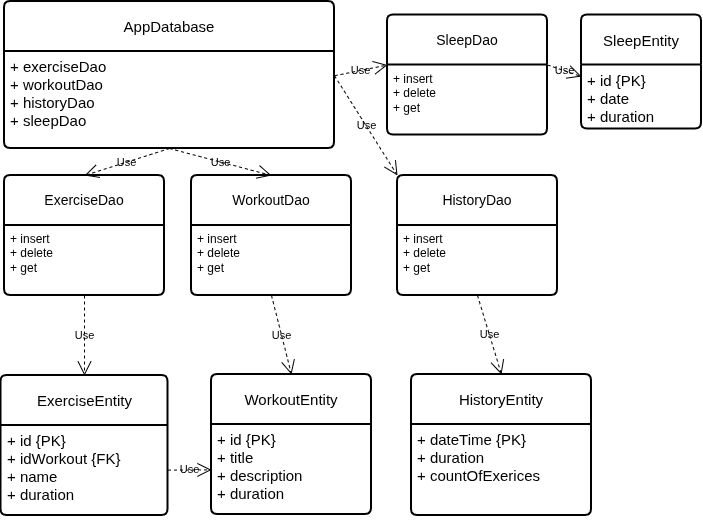
\includegraphics[width=1\textwidth]{images/diagrams/Диаграмма классов бд.png}
    \caption{Диаграмма классов базы данных}
    \label{fig:db_classes}
\end{figure}

\subsubsection{DAO-интерфейсы}

Каждый DAO определяет методы доступа к данным с аннотациями Room:
\begin{itemize}
    \item \texttt{ExerciseDao} — методы вставки, удаления, а также запрос на получение всех упражнений для заданной тренировки.
    \item \texttt{WorkoutDao} — методы вставки, удаления, получения всех тренировок, получения тренировки по идентификатору.
    \item \texttt{SleepDao} — методы вставки, обновления, удаления, получения всех записей сна, получения записей сна за диапазон дат.
    \item \texttt{HistoryDao} — методы вставки, получения всей истории тренировок.
\end{itemize}
Room автоматически генерирует реализации этих интерфейсов.

\subsubsection{Интеграция с Koin}

Все зависимости регистрируются в контейнере Koin. Для каждого компонента указаны его конструкторные параметры.

\paragraph{Сетевые сервисы (API)} — создаются через Retrofit:
\begin{itemize}
    \item \texttt{ExerciseApiService} — получает экземпляр \texttt{Retrofit}.
    \item \texttt{HistoryApiService} — зависит от \texttt{Retrofit}.
    \item \texttt{WorkoutApiService} — зависит от \texttt{Retrofit}.
    \item \texttt{SleepApiService} — зависит от \texttt{Retrofit}.
    \item \texttt{UserApiService} — зависит от \texttt{Retrofit}.
\end{itemize}
Для \texttt{Retrofit} предварительно регистрируется \texttt{OkHttpClient} с интерцепторами (логирование, добавление JWT-токена).

\paragraph{DAO (Data Access Objects)} — получаются из базы данных Room:
\begin{itemize}
    \item \texttt{ExerciseDao} — зависит от \texttt{AppDatabase}.
    \item \texttt{WorkoutDao} — зависит от \texttt{AppDatabase}.
    \item \texttt{SleepDao} — зависит от \texttt{AppDatabase}.
    \item \texttt{HistoryDao} — зависит от \texttt{AppDatabase}.
\end{itemize}
\texttt{AppDatabase} регистрируется как синглтон через \texttt{Room.databaseBuilder()}.

\paragraph{Локальные репозитории} — реализуют интерфейсы из слоя domain, работают только с БД:
\begin{itemize}
    \item \texttt{LocalWorkoutRepositoryImpl} — зависит от \texttt{WorkoutDao} и \texttt{ExerciseDao}.
    \item \texttt{LocalSleepRepositoryImpl} — зависит от \texttt{SleepDao}.
    \item \texttt{LocalHistoryRepositoryImpl} — зависит от \texttt{WorkoutDao} и \texttt{ExerciseDao}.
    \item \texttt{LocalUserRepositoryImpl} — зависит от \texttt{SharedPreferences} (хранилище токена).
\end{itemize}

\paragraph{Удалённые репозитории} — реализуют интерфейсы из слоя domain, работают только с API:
\begin{itemize}
    \item \texttt{ExerciseRemoteRepositoryImpl} — зависит от \texttt{ExerciseApiService}.
    \item \texttt{HistoryRemoteRepositoryImpl} — зависит от \texttt{HistoryApiService}.
    \item \texttt{WorkoutRemoteRepositoryImpl} — зависит от \texttt{WorkoutApiService}.
    \item \texttt{SleepRemoteRepositoryImpl} — зависит от \texttt{SleepApiService}.
    \item \texttt{UserRemoteRepositoryImpl} — зависит от \texttt{UserApiService}.
\end{itemize}

\paragraph{ViewModel} — управляют UI, получают необходимые репозитории (локальные или удалённые) через конструктор:
\begin{itemize}
    \item \texttt{MainViewModel} — зависит от \texttt{LocalWorkoutRepository} и \texttt{LocalSleepRepository} (или от use case, который их объединяет).
    \item \texttt{TrainingViewModel} — зависит от \texttt{LocalWorkoutRepository} и \texttt{ExerciseRepository}.
    \item \texttt{SleepTrackerViewModel} — зависит от \texttt{LocalSleepRepository} и \texttt{SleepRecommendationUseCase}.
    \item \texttt{HistoryViewModel} — зависит от \texttt{LocalHistoryRepository}.
    \item \texttt{ProfileViewModel} — зависит от \texttt{LocalUserRepository} и \texttt{LocalWorkoutRepository}.
    \item \texttt{AuthViewModel} — зависит от \texttt{UserRemoteRepository} (или use case для аутентификации).
\end{itemize}

Регистрация выполняется с помощью функций \texttt{singleOf(...)} и \texttt{viewModelOf(...)}. Например:
\begin{verbatim}
singleOf(::LocalWorkoutRepositoryImpl) { bind<LocalWorkoutRepository>() }
singleOf(::WorkoutRemoteRepositoryImpl) { bind<WorkoutRemoteRepository>() }
viewModelOf(::MainViewModel)
\end{verbatim}

\subsubsection{Преобразования между Entity и Domain}

Для каждого Entity определена функция расширения \texttt{toDomain()}, которая создаёт доменную модель. Доменные модели имеют аналогичные функции \texttt{toEntity()}. Это позволяет репозиториям не загромождаться логикой маппинга.

\subsection{Логика отображения тренировок, прогресса, сна и советов}

За отображение данных отвечают ViewModel, которые взаимодействуют с репозиториями (локальными или удалёнными) и поставляют состояние UI через Compose. Каждый экран имеет свою ViewModel. Все ViewModel получают зависимости через конструктор и регистрируются в Koin.

\begin{itemize}
    \item \texttt{MainViewModel} — отвечает за главный экран со списком тренировок. Получает \texttt{LocalWorkoutRepository} и \texttt{LocalSleepRepository}. При создании загружает список доступных тренировок через \texttt{localWorkoutRepository.getWorkouts()} и подписывается на изменения. Также предоставляет метод для получения рекомендации на основе последних записей о сне (через \texttt{localSleepRepository.getAverageSleepForLastWeek()}).

    \item \texttt{TrainingViewModel} — управляет процессом активной тренировки. Получает \texttt{LocalWorkoutRepository} и \texttt{ExerciseRemoteRepository} (для получения полного списка упражнений). Хранит состояние текущего упражнения, таймер, список оставшихся упражнений. Предоставляет методы \texttt{startTraining()}, \texttt{pauseTraining()}, \texttt{finishTraining()}, \texttt{nextExercise()}. При завершении тренировки сохраняет результат через \texttt{localWorkoutRepository.saveWorkout()}.

    \item \texttt{SleepTrackerViewModel} — отвечает за экран трекера сна. Получает \texttt{LocalSleepRepository}. Загружает историю записей о сне через \texttt{localSleepRepository.getSleepRecords()}. Предоставляет методы для добавления, редактирования и удаления записи. Также вычисляет статистику (средний сон за неделю, график) и генерирует текстовые советы через \texttt{SleepRecommendationUseCase}.

    \item \texttt{HistoryViewModel} — для экрана истории тренировок. Получает \texttt{LocalHistoryRepository}. Загружает список завершённых тренировок и предоставляет методы для фильтрации по дате.

    \item \texttt{ProfileViewModel} — для экрана профиля пользователя. Получает \texttt{LocalUserRepository} и \texttt{LocalWorkoutRepository}. Отображает имя пользователя, общую статистику (количество тренировок, общее время). Предоставляет метод \texttt{logout()}, который очищает токен и перенаправляет на экран входа.

    \item \texttt{AuthViewModel} — для экранов входа и регистрации. Получает \texttt{UserRemoteRepository} (удалённый репозиторий для аутентификации). Предоставляет методы \texttt{login(username, password)} и \texttt{register(username, password, displayName)}. При успешной аутентификации сохраняет токен через \texttt{LocalUserRepository} и обновляет состояние.
\end{itemize}

Регистрация ViewModel в Koin:
\begin{verbatim}
viewModelOf(::MainViewModel)
viewModelOf(::TrainingViewModel)
viewModelOf(::SleepTrackerViewModel)
viewModelOf(::HistoryViewModel)
viewModelOf(::ProfileViewModel)
viewModelOf(::AuthViewModel)
\end{verbatim}

Все ViewModel используют \texttt{viewModelScope} для запуска корутин, что обеспечивает автоматическую отмену задач при уничтожении ViewModel. Данные отображаются с использованием Jetpack Compose: списки тренировок и упражнений — через \texttt{LazyColumn}, графики сна — через кастомные composable, статистика — через текстовые поля. Прогресс (например, количество выполненных тренировок за неделю) вычисляется в ViewModel на основе данных из репозиториев и отображается в виде индикаторов (прогресс-бары, круговые диаграммы). Советы выводятся в виде текстовых карточек на главном экране и в разделе сна.

\subsection{Реализация модуля анализа тренировок и сна для формирования советов}

Для выработки персонализированных подсказок разработаны два независимых алгоритма, размещённых в доменном слое (пакет \texttt{domain/usecase}). Данные компоненты не привязаны к платформенно-зависимым Android-библиотекам, что обеспечивает их чистоту и тестируемость.

\paragraph{Анализ стабильности тренировок:}
На основе накопленной истории завершённых занятий вычисляется показатель регулярности. Use case под названием \texttt{TrainingStabilityUseCase} получает на вход перечень выполненных тренировок за последние 1–2 недели (7–14 дней) и оценивает частоту пропусков или преждевременных завершений. Принятые правила:
\begin{itemize}
    \item если пользователь успешно закрывает запланированные занятия без единого пропуска на протяжении пяти и более циклов подряд, система сигнализирует о возможности повышения нагрузки — например, увеличить число подходов, продлить длительность или добавить рабочий вес;
    \item при двух и более пропущенных тренировках подряд алгоритм предлагает снизить объём (уменьшить количество упражнений) или ослабить интенсивность;
    \item в ситуациях, когда более 30\% тренировок за неделю не были доведены до конца (пользователь прервал их досрочно), система рекомендует сократить либо число упражнений, либо их продолжительность — чтобы сделать план более реалистичным;
    \item во всех прочих случаях нагрузка остаётся без корректировок.
\end{itemize}
Сгенерированная рекомендация передаётся в \texttt{MainViewModel} и отображается на главном экране в формате короткого текстового сообщения.

\paragraph{Анализ продолжительности сна:}
Репозиторий \texttt{SleepRepository} предоставляет метод \texttt{getAverageSleepForLastWeek()}, который рассчитывает среднесуточную длительность сна за последние семь дней. Use case \texttt{SleepRecommendationUseCase}, опираясь на это среднее значение, формирует одну из следующих подсказок:
\begin{itemize}
    \item если сон в среднем длится менее 6 часов — «Для полноценного восстановления старайтесь спать 7–8 часов»;
    \item при значении от 6 до 7 часов (менее 7) — «Постарайтесь увеличить ночной сон на 30–60 минут»;
    \item в диапазоне 7–9 часов — «Вы отлично высыпаетесь, поддерживайте режим»;
    \item при сне более 9 часов — «Возможна пересып, попробуйте сократить отдых на 15–30 минут».
\end{itemize}
Кроме того, реализована комбинированная логика: если средняя продолжительность сна опускается ниже 6,5 часа и при этом недельная тренировочная нагрузка превышает 4 занятия, система выдаёт совет снизить интенсивность либо добавить дополнительный день отдыха. Данная логика вынесена в отдельный метод \texttt{getCombinedRecommendation()}, который объединяет результаты обоих анализов.

\subsection{Реализованное решение}

По итогам выполнения всех этапов создано приложение, выполняющее роль интеллектуального помощника в фитнесе. Полный исходный код вынесен в приложение 2. Ключевые характеристики разработанной системы:

\begin{itemize}
    \item \textbf{Гибкость построения тренировок}. Вместо жёстких линейных сценариев каждая тренировочная сессия представляет собой самостоятельный набор упражнений. Пользователь может произвольно редактировать состав упражнений внутри сеанса, адаптируя нагрузку под текущее самочувствие, доступное время или актуальные цели.
    
    \item \textbf{Адаптивный механизм коррекции нагрузки}. Анализируя историю завершённых занятий, приложение даёт персонализированные подсказки: при стабильном выполнении плана предлагается повысить нагрузку; при систематических пропусках или незавершённых тренировках — уменьшить число упражнений либо сократить их длительность.
    
    \item \textbf{Встроенный трекер сна с обратной связью}. Пользователь вручную вносит данные о продолжительности сна, и система учитывает эту информацию при выработке советов. Недостаток сна служит сигналом для снижения тренировочной нагрузки и увеличения времени отдыха.
    
    \item \textbf{Модуль совместного анализа тренировок и сна для выработки рекомендаций}. Данный модуль объединяет два направления: на основе истории тренировок вычисляется регулярность выполнения плана, а по записям о сне — средняя длительность ночного отдыха. На пересечении этих метрик формируются текстовые советы, которые выводятся на главном экране и в разделе сна.
\end{itemize}

Разработанное приложение включает в себя:
\begin{itemize}
    \item каталог готовых тренировочных комплексов с возможностью настройки;
    \item инструмент для создания собственных тренировочных планов;
    \item экран проведения тренировки с таймером и возможностью включения фонового аудио;
    \item полную историю всех проведённых занятий;
    \item трекер сна со статистическими сводками и рекомендациями.
\end{itemize}

Дополнительно создано серверное приложение, обеспечивающее регистрацию пользователей и аутентификацию на основе токенов.

Таким образом, реализованное решение замыкает контур обратной связи «нагрузка → восстановление → рекомендация → корректировка нагрузки», что позволяет динамически адаптировать тренировочный процесс под индивидуальные особенности и текущее состояние пользователя.